%%%%%%%
% Ch4 %
%%%%%%%

\chapter{Ponts universels}
	\begin{wrapfigure}[5]{l}{6 cm}
	\vspace{-5mm}
	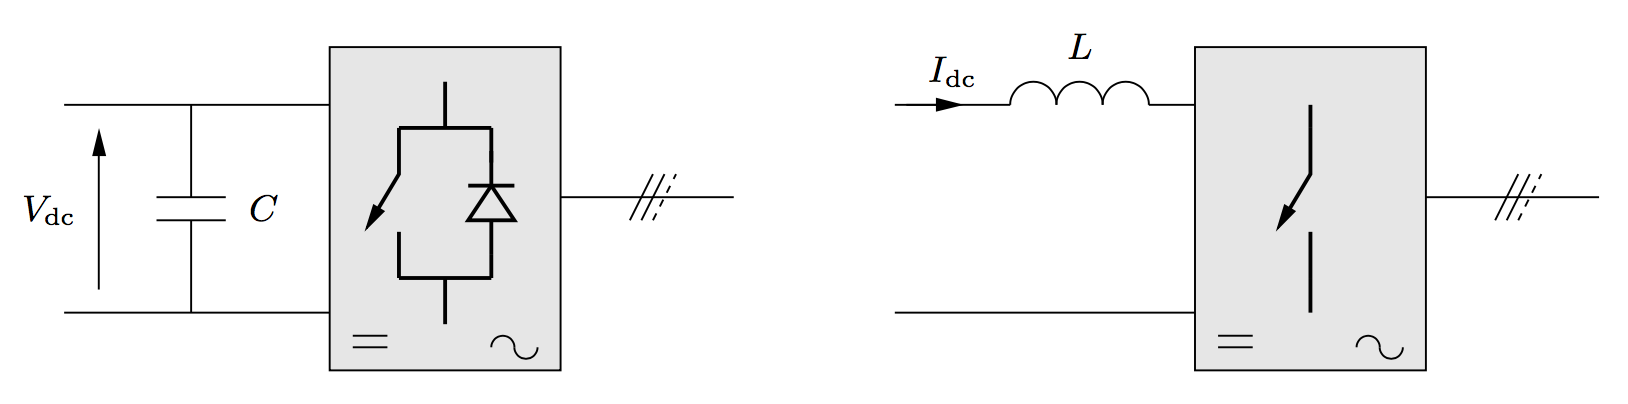
\includegraphics[scale=0.2]{ch4/1}
	\captionof{figure}{}
	\end{wrapfigure}
	Les \textbf{onduleurs autonomes} possèdent généralement une structure en pont et sont constitués d'interrupteurs commandables. Ils peuvent être alimentés par une source de tension continue (voltage source converter, VSC) ou par une source de courant continu (CSC), les deux modèles diffèrent par un condensateur ou une inductance dans le bus d'entrée. Ils peuvent fonctionner en \textbf{redresseur}. Les hacheurs \textbf{multi quadrants} utilisés entre autres pour la commande de moteur à courant continu ont la même topologie avec une commande semblable. 
	
	\begin{minipage}{0.5\textwidth}
		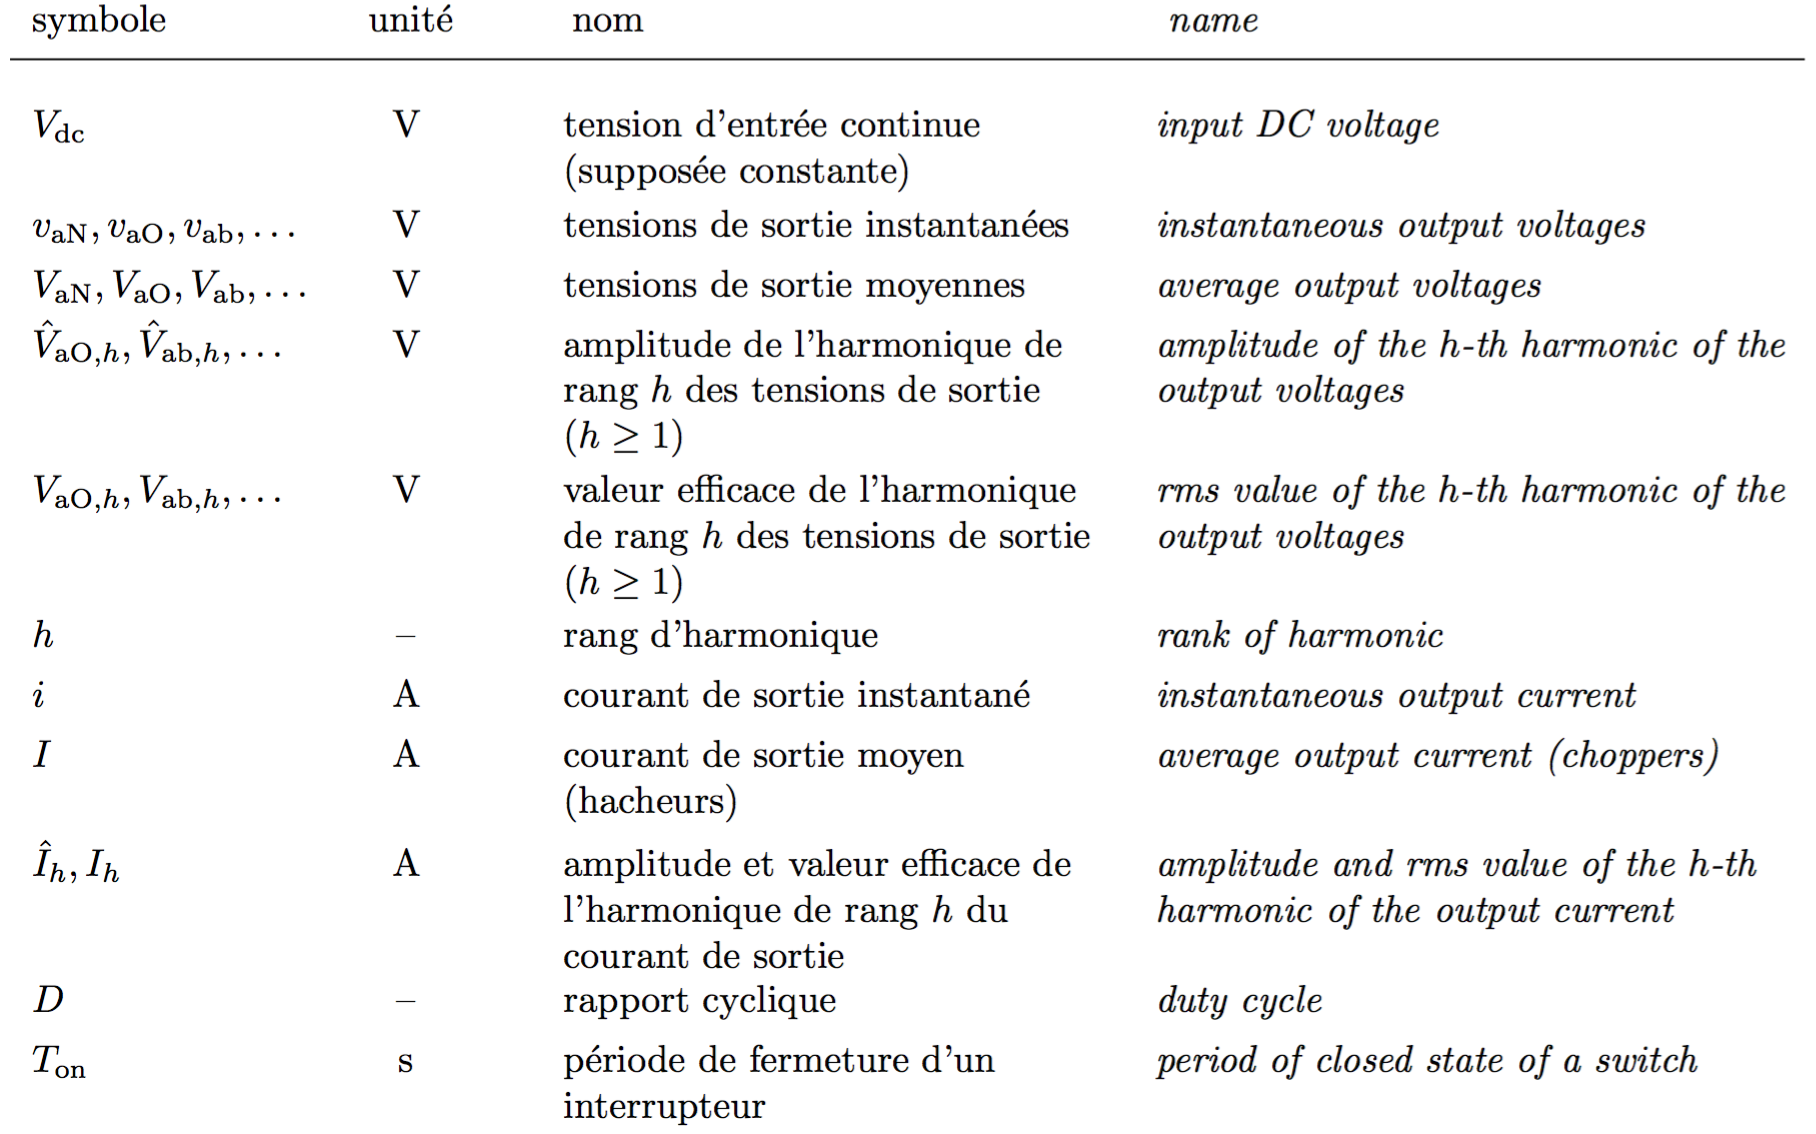
\includegraphics[scale=0.25]{ch4/2}
	\end{minipage}
	\begin{minipage}{0.5\textwidth}
		\vspace{3mm}
		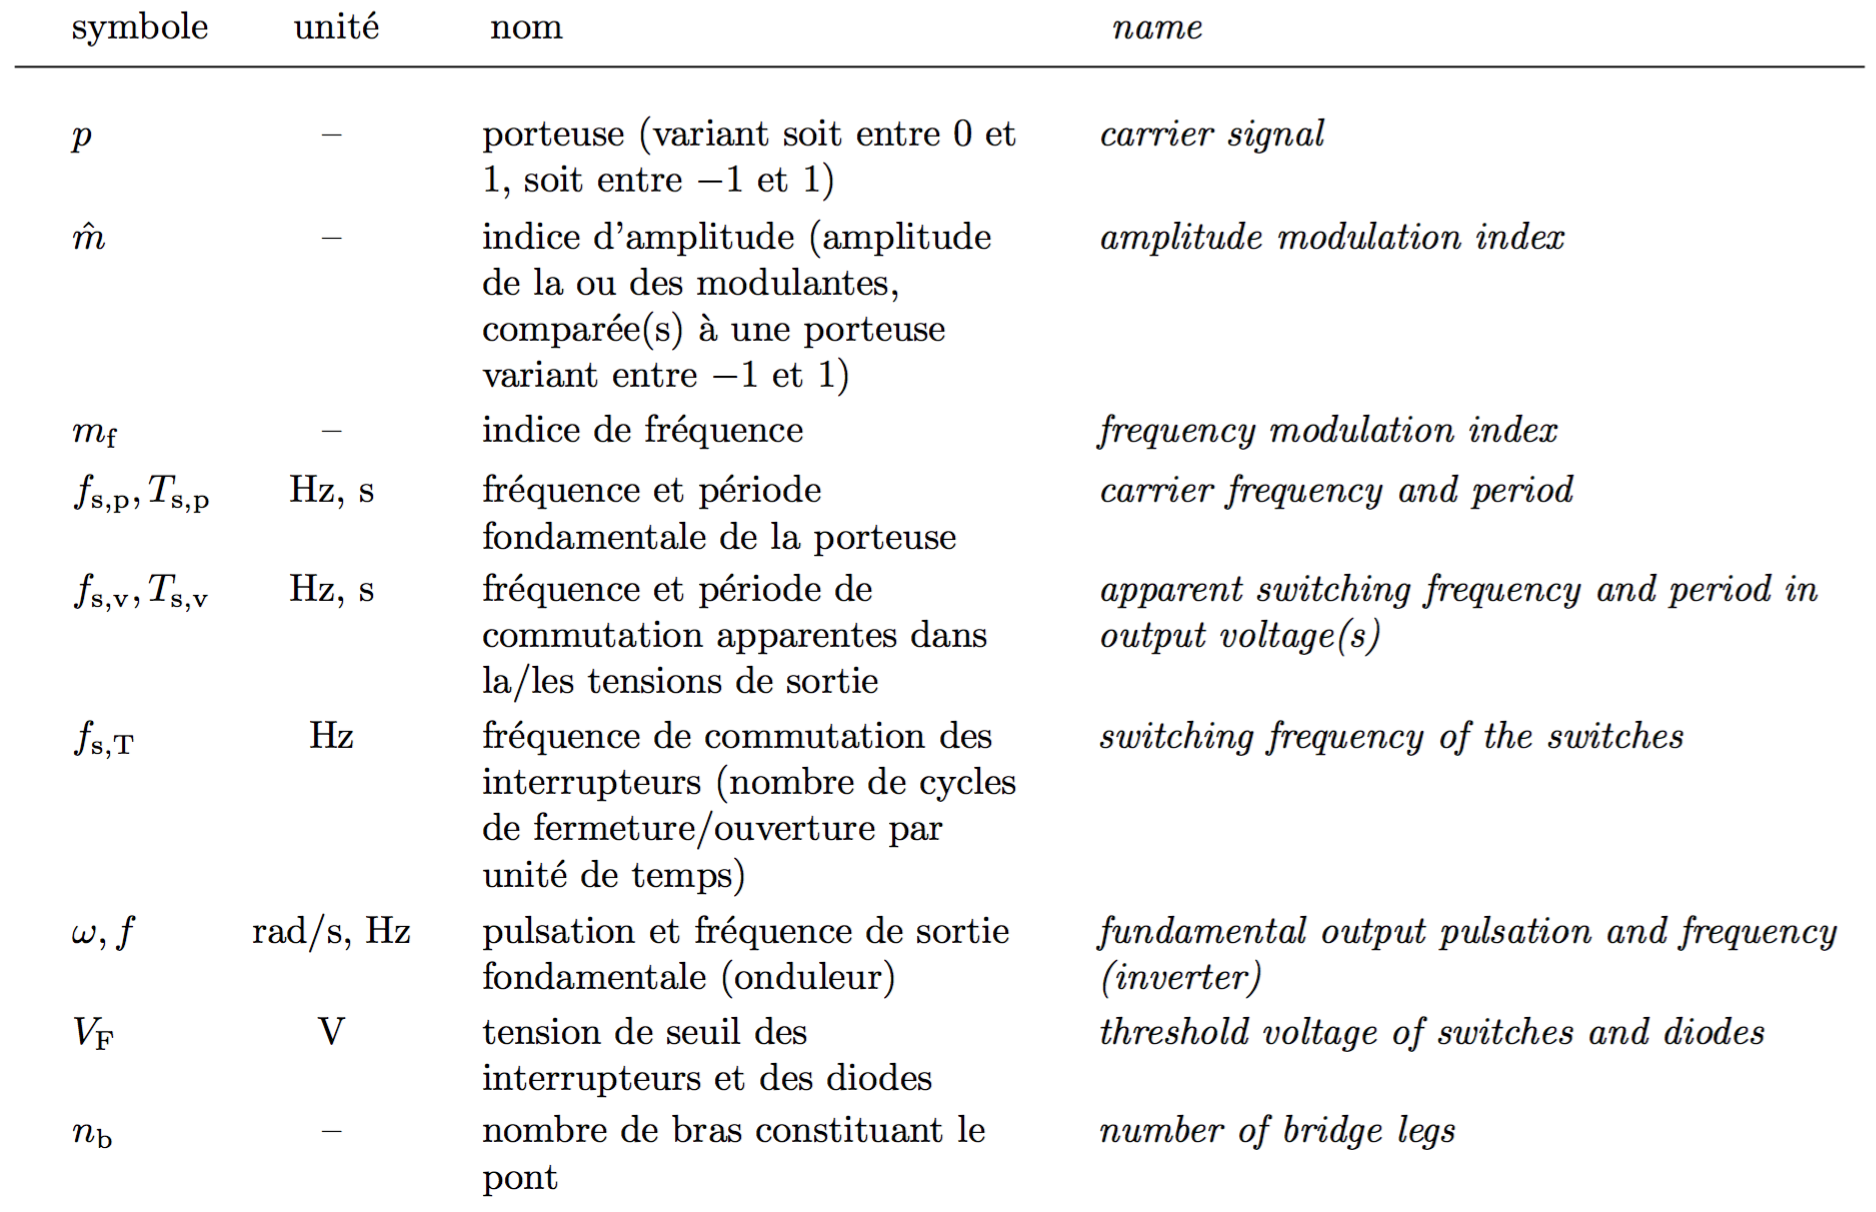
\includegraphics[scale=0.25]{ch4/3}	
	\end{minipage}
	\captionof{table}{Liste des abréviations et symboles.}
	
\section{Caractéristiques des interrupteurs commandables}
	\begin{wrapfigure}[4]{r}{5 cm}
	\vspace{-5mm}
	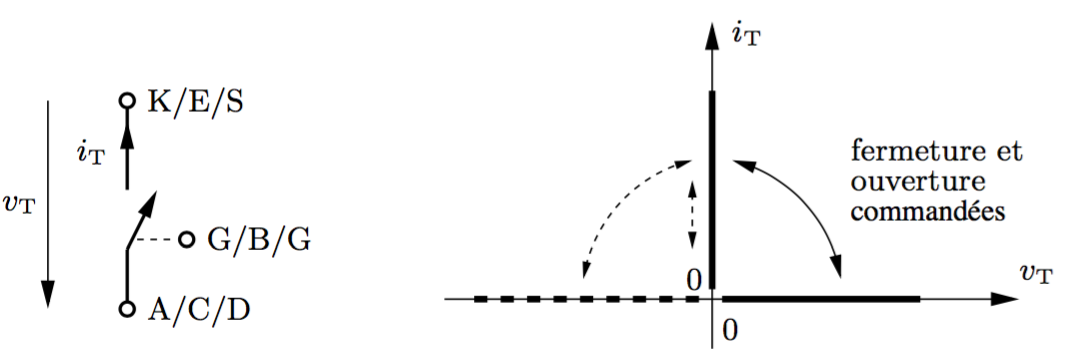
\includegraphics[scale=0.25]{ch4/4}
	\captionof{figure}{}
	\end{wrapfigure}
	Ci-contre, la caractéristique tension-courant idéalisée d'un interrupteur commandable. Le 2${ème}$ quadrant ne nous intéresse pas puisque la tension $v_T$ y est négative et est exclue lorsqu'une diode est raccordée en antiparallèle sur l'interrupteur. \\
	
	\begin{wrapfigure}[6]{l}{6 cm}
	\vspace{-5mm}
	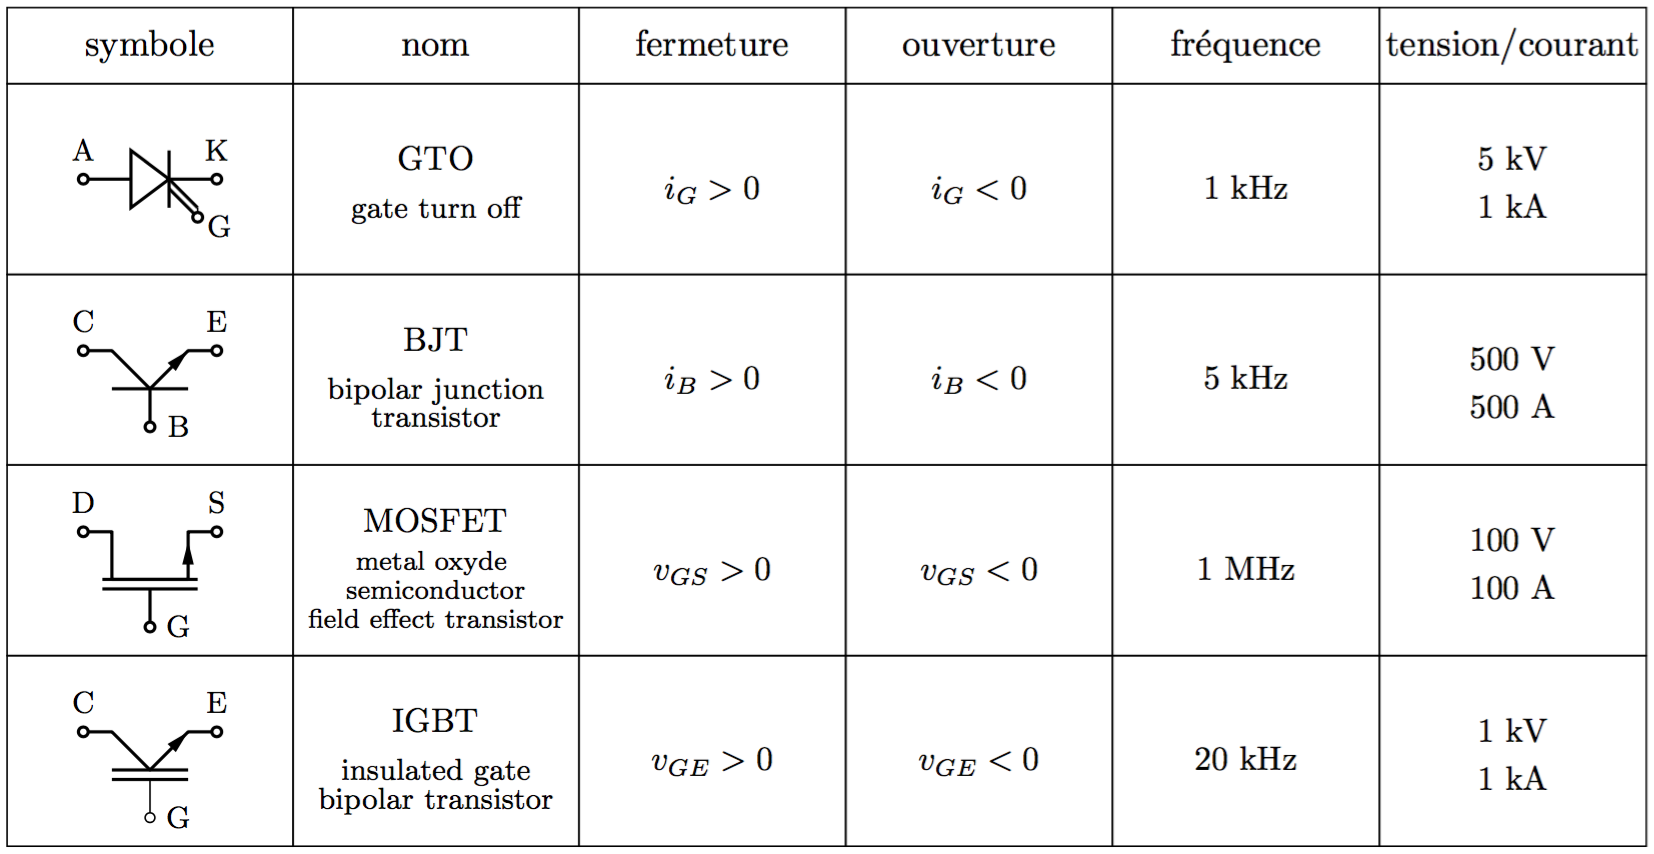
\includegraphics[scale=0.2]{ch4/5}
	\captionof{figure}{}
	\end{wrapfigure}
	Ils sont tous \textbf{unidirectionnels} donc le courant ne peut circuler que de l'anode A vers la cathode K, du collecteur C vers l'émetteur E ou du drain D vers la source S. L'\textbf{électrode de commande} (gâchette G, base B ou grille G) permet d'effectuer la fermeture et ouverture de l'interrupteur grâce à une tension ou un courant. 
	
	La tension $V_{T,max}$ et le courant $I_{T,max}$ maximum supportés ou conduits par l'interrupteur sont limités. On peut faire des montages en série ou en parallèle pour augmenter la puissance nominale, mais il va falloir faire une répartition uniforme du courant et tension. La commutation entre l'état passant et bloqué prend un certain temps plus ou moins important, ce qui limite la fréquence de commutation $f_{s,T}$. Durant ces intervalles, la tension et le courant sont tous deux importants et donnent lieu à des \textbf{pertes de commutation}.
	
\section{Convertisseurs à source de tension : généralités}
	\subsection{Topologie et réalisation pratique}	
		\begin{wrapfigure}[12]{l}{7cm}
		\vspace{-5mm}
		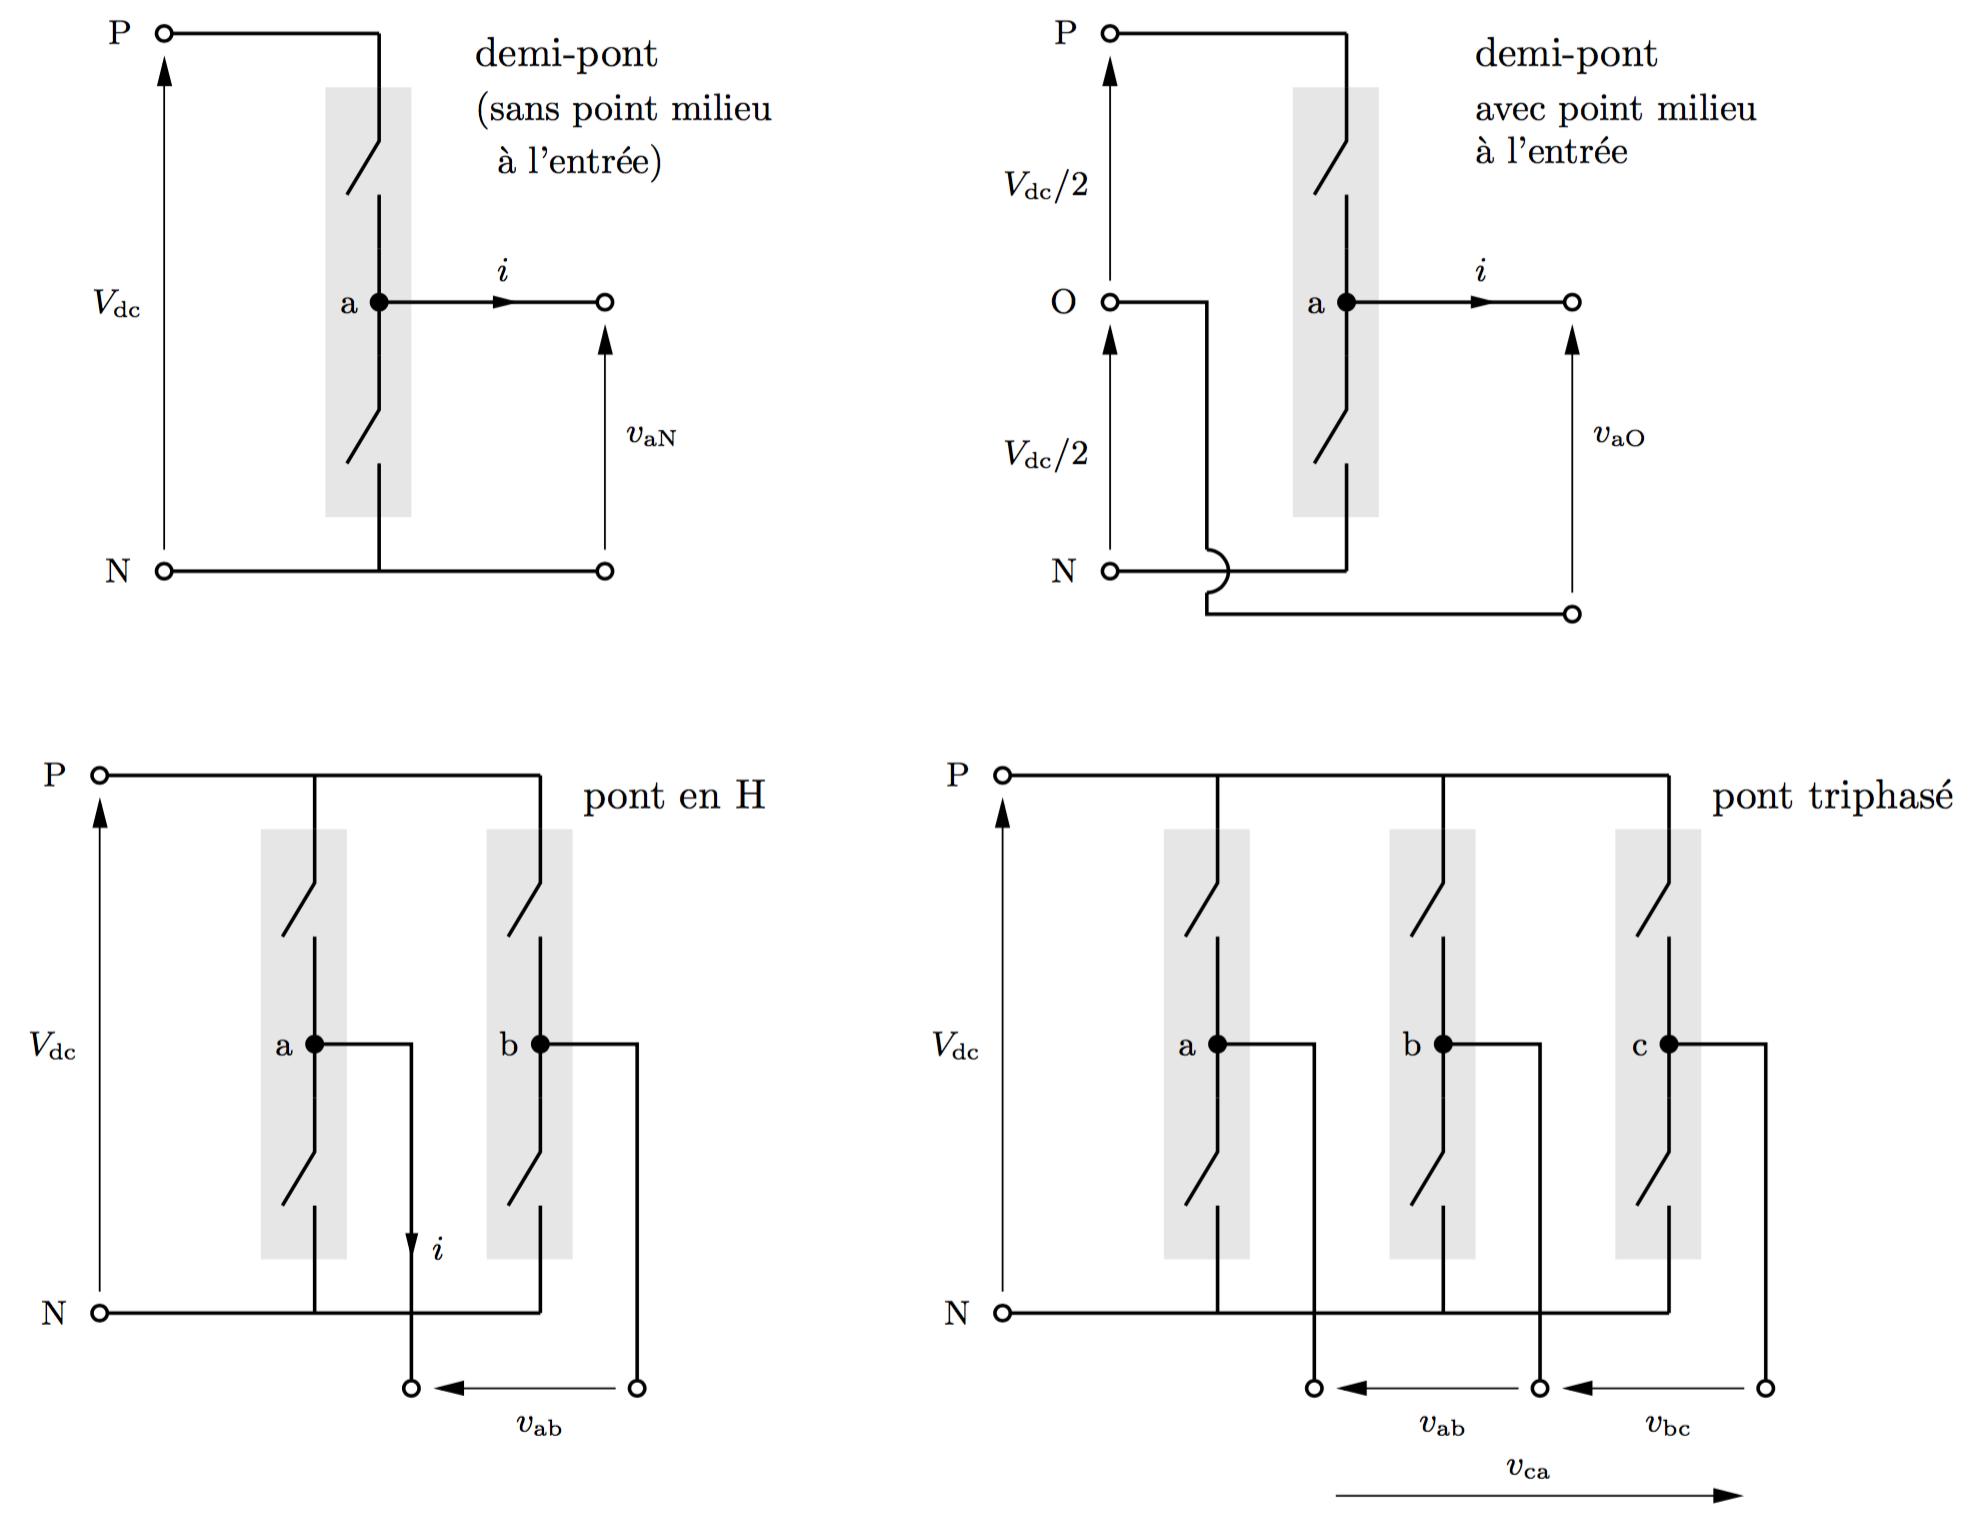
\includegraphics[scale=0.2]{ch4/7}
		\captionof{figure}{}
		\end{wrapfigure}
		La figure ci-contre reprend 4 topologies de ponts à 1,2 ou 3 bras. Chaque bras comprend un interrupteur bidirectionnel en courant et commandable et est relié entre les pôles N et P de l'entrée. Les points milieux a, b et c constituent les bornes de sortie, ainsi que N et O dans le demi-pont. Pour éviter un court-circuit, les 2 interrupteurs d'un même bras de peuvent être fermés en même temps, sous risque de détruire les interrupteurs. En jouant avec les interrupteurs, on forme des tensions de sortie différentes. \\
		
		Pour le premier demi-pont, on a $v_{aN} = 0$ ou $v_{aN} = V_{dc}$. Dans le second, $v_{aN} = \pm V_{dc}/2$. Pour les deux derniers, $v_{aN} = 0$ ou $v_{aN} = \pm V_{dc}$. On peut donc fabriquer une ou des tensions continues ou alternatives de valeur moyenne désirée.  
		
		\begin{wrapfigure}[9]{r}{4cm}
		\vspace{-5mm}
		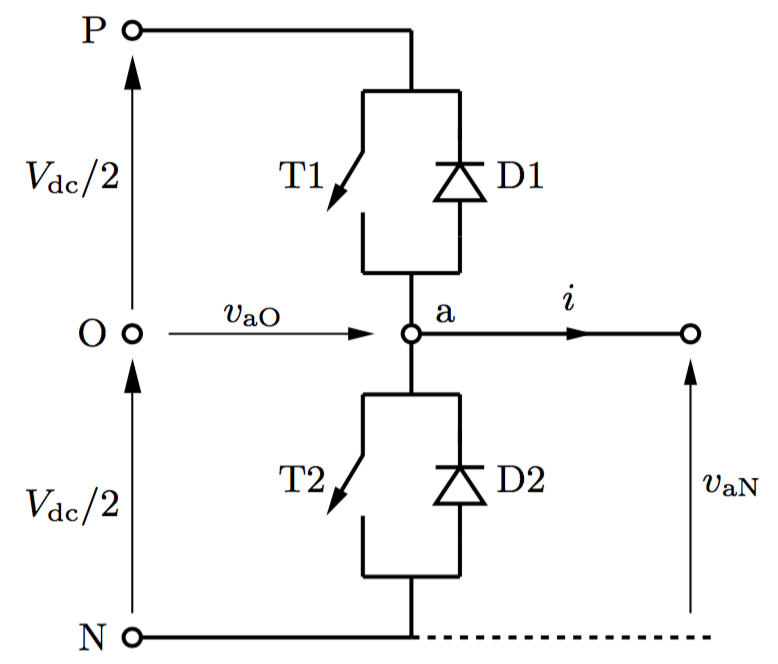
\includegraphics[scale=0.3]{ch4/8}
		\captionof{figure}{}
		\end{wrapfigure}
		\ \\ Ci-contre on peut voir que chaque bras est constitué de 2 interrupteurs commandables et unidirectionnels en courant (GTO, BJT, IGBT, MOSFET, ...), T1 et T2 et de 2 diodes de roue libre, D1 et D2 en  antiparallèle sur les interrupteurs. Pour éviter le court-circuit via les 2 diodes, il faut impérativement que la tension d'entrée soit \textbf{positive}. Si T1 est fermé, T2 doit être ouvert, a est alors relié à P et D2 est polarisé en inverse. Si $i>0$, il circulera dans T1 sinon dans D1. Pareil si T2 est fermé, T1 est ouvert et a est raccordé à N, D1 est polarisé en inverse. Si $i>0$ il passe dans D2, sinon dans T2. \\
		
		Intéressons-nous à $v_{aO}(t)$ du demi-pont en supposant $V_{dc}<0$ et cst. $v_{aO}(t)$ ne dépend que de l'état des interrupteurs, si T1 est fermé, $v_{aO(t)} = + V_{dc}/2$ et si T2 est fermé $v_{aO}(t) = -V_{dc}/2$, quel que soit le signe du courant. On peut donc, en jouant sur l'intervalle de fermeture des T obtenir une consigne moyenne entre $+V_{dc}/2$ et $-V_{dc}/2$. \\
		
		Vu la vitesse de commutation, il faut intercaler un petit intervalle de temps ou les 2 T sont ouverts en même temps pour éviter le court-circuit. On parle de temps mort (dead time) $t_{\Delta}$. Durant $t_{\Delta}$, c'est le signe du courant qui détermine $v_{aO}$. 
		
	\subsection{Conduction dans les composants semi-conducteurs et pertes associées}
		\begin{wrapfigure}[8]{l}{5.5cm}
		\vspace{-5mm}
		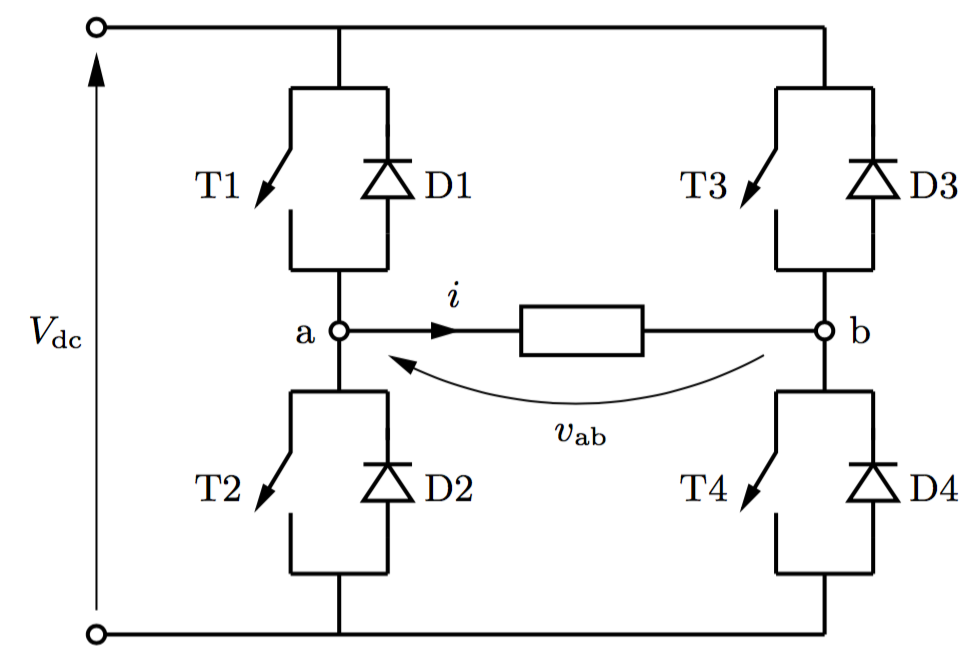
\includegraphics[scale=0.3]{ch4/9}
		\captionof{figure}{}
		\end{wrapfigure}
		Lorsque les interrupteurs conduisent, il y a la \textbf{tension résiduelle} faible, mais non nulle à leurs bornes (1 à 3V), donnant lieu aux pertes de conduction. En état ouvert, le courant de fuite est négligeable. Selon les états ouvert et fermé, 2 fois neuf combinaisons existent (4 $\times$ états complémentaires, 4 $\times$ un bras sans fermeture et l'état tous ouverts). Pour exemple, si la conduction se fait au travers D2 et D3 dans un pont en H, il vient :
		\begin{equation}
			V_{ab} = -V_{dc}-V_{F,D2}-V_{F,D3}-(R_{on,D2}+R_{on,D3})i,
		\end{equation}
		où les pertes de conduction instantanées (en W) s'obtiennent en multipliant la seconde partie par $i$. A courant négatif, à conduction dans T2 et T3 on a :
		\begin{equation}
			V_{ab} = -V_{dc}+V_{F,T2}+V_{F,T3}-(R_{on,T2}+R_{on,T3})i. 
		\end{equation}
		
	\subsection{Commutation dans un bras et pertes associées}
		\begin{wrapfigure}[8]{r}{8cm}
		\vspace{-5mm}
		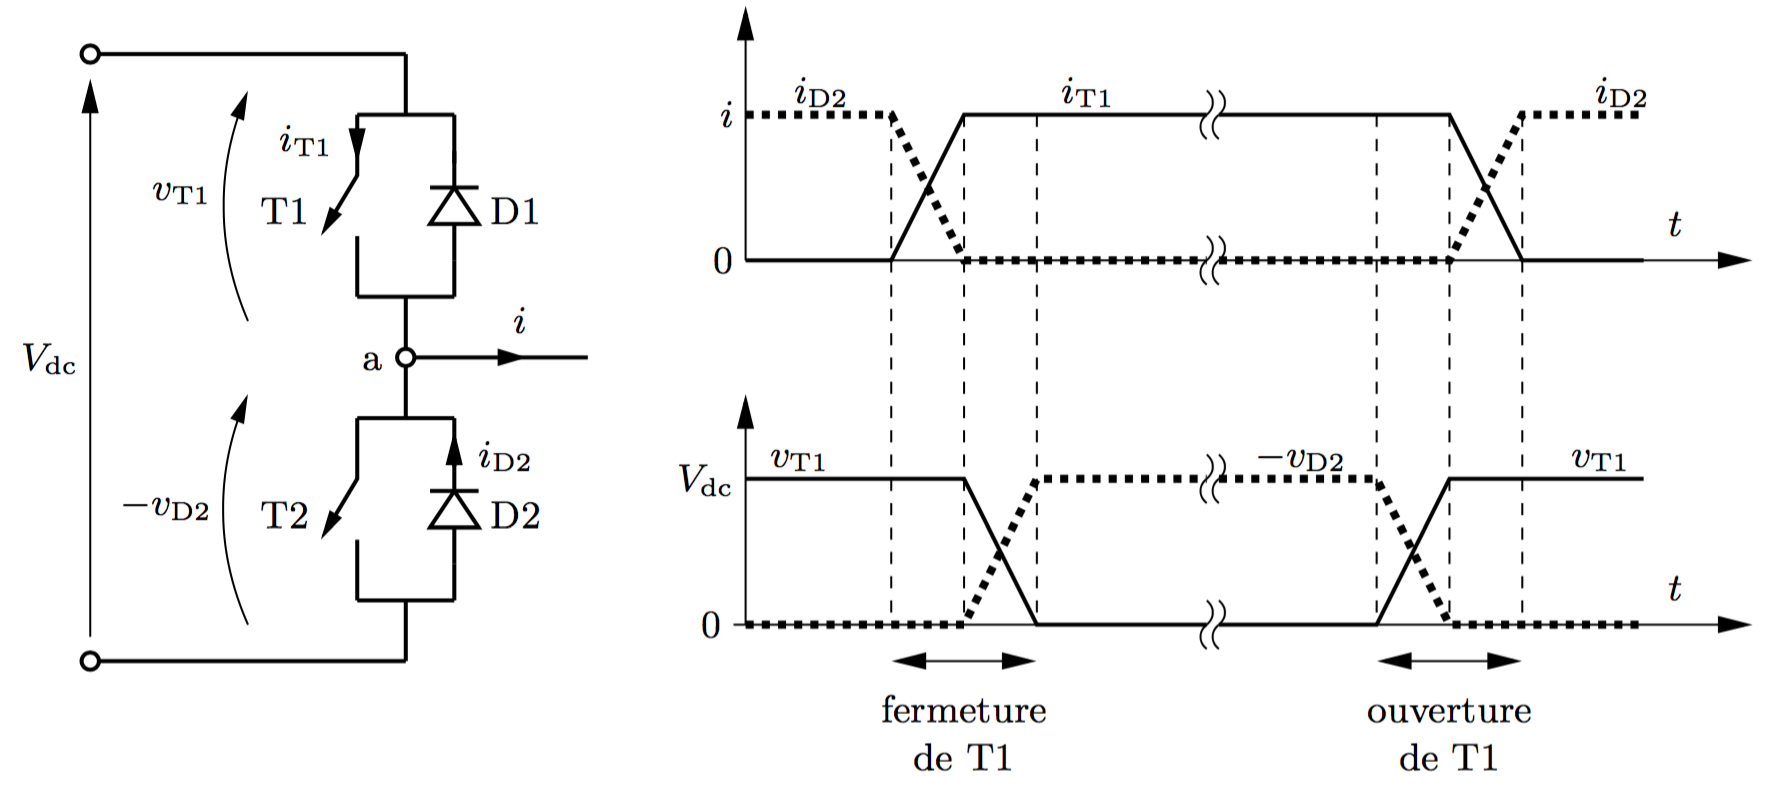
\includegraphics[scale=0.25]{ch4/10}
		\captionof{figure}{}
		\end{wrapfigure}
		Considérons un demi-pont dont le point milieu est connecté à une charge inductive, le courant ne pouvant varier que lentement et circule entièrement soit dans T1 soit D2 ou les 2 durant la commutation : 
		\begin{equation}
			i = i_{T1}+ i_{D2}.
		\end{equation}		 
		Du côté de la tension :
		\begin{equation}
			V_{dc} = v_{T1} - v_{D2},
		\end{equation}
		où $v_{T1}$ et $v_{D2}$ sont pratiquement nulle en conduction et égal à $V_{dc}$ et $-V_{dc}$ en non-conduction et varient entre les 2 valeurs en commutation. Les formes d'onde nous indiquent que, lorsque la fermeture de T1 est commandée, $i_{T1}$ croît à partir de 0 alors que D2 continue à conduire avec $v_{D2} = 0$ et $v_{T1} = V_{dc}$. Ce n'est que lorsque D2 s'arrête de conduire que $-v_{D2}$ peut monter jusque $V_{dc}$ et $v_{T1}$ chuter jusque 0. Pour son ouverture, il faut $v_{T1}$ monte jusque $V_{dc}$ pour que D2 se retrouve polarisé en direct et puisse conduire. \\
		
		Durant la commutation, $p_{T1} = v_{T1}i_{T1}$ est non négligeable et l'intégrale sur un intervalle de commutation donne une énergie d'autant plus grande que $V_{dc}, i$ et les temps de commutations sont grands. On en vient à introduire alors la fréquence de commutation. Sur base des données dans les datasheets, les pertes de commutation dans les bras (en W) peuvent être approchées comme :
		\begin{equation}
			P_{com} = f_{s,T} (E_{on,ref}+ E_{off,ref})\frac{V_{dc}}{V_{dc,ref}}\frac{i}{i_{ref}},
		\end{equation}
		où les E sont les énergies susmentionnées relatives aux valeurs de référence.
	
\section{Hacheurs - modulation de largeur d'impulsions (MLI)}
	 \textbf{Pulse width modulation (PWM)} est une des méthodes de commande des bras du convertisseur. La fréquence de commutation est maintenue constante et pour chaque bras, la période de commutation est scindée en 2 parties où c'est d'abord l'interrupteur supérieur qui est fermé puis l'inférieur. En modulant la durée des sous-intervalles, on génère la tension moyenne. \\
	 
	 Les tensions sont entachées d'une série d'harmoniques en raison de la commutation. Les charges inductives font que les courants sont en meilleur état. Notons qu'en cas de commande à hystérésis, la fréquence de commutation n'est pas constante et les harmoniques sont alors de fréquence variable (problème du filtre). \\
	 La \textbf{MLI intersective} consiste à déterminer les instants de commutation pour un bras en comparant la \textbf{porteuse p(t)}, signal triangulaire de fréquence $f_{s,p}$ et la \textbf{modulante}, image de la tension souhaitée. Pour les ponts en H dans le cas monophasé, il est possible d'utiliser la même modulante pour les 2 bras (modulation bipolaire) ou d'en prendre 2 séparés (modulation unipolaire) avec la même porteuse. Pour un pont onduleur/redresseur \textbf{triphasé}, il faut considérer trois modulantes formant un système triphasé équilibré. \\
	 
	 Lorsque la commande est faite avec de l'électronique analogique, la comparaison de p(t) et m(t) est faite telle quelle. Avec de l'électronique digitale, même résultat obtenu sans réelle comparaison (rapport cyclique). 
	 
	 \subsection{Demi-pont}
	 	\subsubsection{Sans point milieu à l'entrée}
	 		\begin{wrapfigure}[8]{l}{6.5cm}
			\vspace{-5mm}
			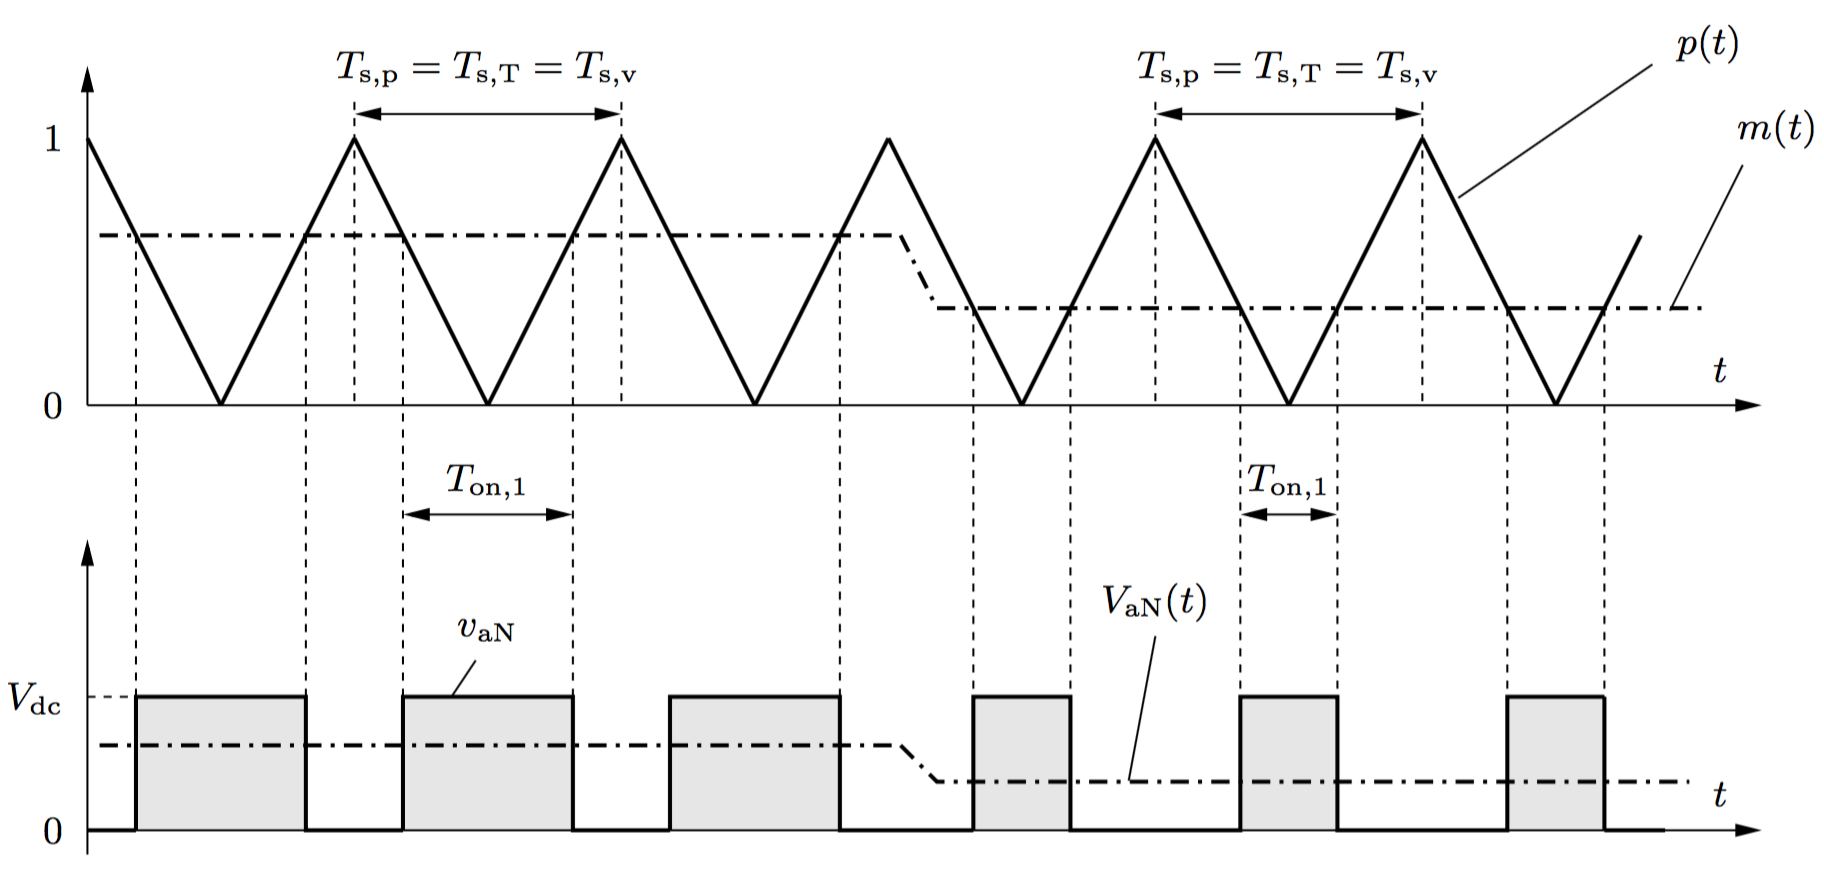
\includegraphics[scale=0.2]{ch4/6}
			\captionof{figure}{}
			\end{wrapfigure}
			Comme la tension de sortie $v_{aN}(t)$ est toujours positive ou nulle, on prend p(t) triangulaire variant entre 0 et 1. La m(t) est supposée varier lentement (constante sur une période de commutation $T_{s,p}$) par rapport à la porteuse. Quand $m(t) > p(t)$, l'interrupteur supérieur du bras est fermé et $v_{aN} = V_{dc}$. Quand $m(t) < p(t)$, c'est l'interrupteur inférieur qui est fermé et $v_{aN}$ = 0. On suppose que la m(t) est aussi comprise entre 0 et 1 de telle manière que p et m se croisent 2x par période de commutation $T_{s,p}$ et les interrupteurs s'ouvrent et se ferment à la même fréquence, qu'on retrouve aussi dans $v_{aN}$ : 
			\begin{equation}
				f_{s,p} = f_{s,T} = f_{s,v}. 
			\end{equation}
			Nous définissons le \textbf{rapport cyclique} (duty cycle) d'un interrupteur comme la fraction du temps pendant laquelle il est fermé $0<D_x<1$. Pour T1 et T2 en négligeant le temps mort cela donne : 
			\begin{equation}
				D_1 = \frac{T_{on,1}}{T_s} \qquad et \qquad D_2 = \frac{T_{on,2}}{T_s} = \frac{T_s - T_{on,1}}{T_s} = 1 - D_1.
			\end{equation}
			Par convention, D d'un bras est celui de son interrupteur supérieur, donc $D = D_1$. Dans le cas présent :
			\begin{equation}
				D(t) = m(t). 
			\end{equation}
			On définit la \textbf{moyenne rapide} de $v_{aN}$ (moyennage sans harmoniques de commutation) : 
			\begin{equation}
				V_{aN}(t) = \frac{1}{T_s}\int _{t-T_s/2}^{t+T_s/2} v_{aN}(t') \, dt'
			\end{equation}
			qui varie lentement par rapport à $T_s$. On retrouve alors  approximativement : 
			\begin{equation}
				V_{aN}(t) = m(t) V_{dc}. 
			\end{equation}
			
		\subsubsection{Avec point milieu à l'entrée}
			Puisque $V_{aO}(t) = V_{aN}(t) - V_{dc}/2$ peut être positive ou négative, il peut fonctionner aussi bien en onduleur/redresseur qu'en hacheur. En prenant le même $p(t)$, on a toujours $D(t) = m(t)$ :
			\begin{equation}
				V_{aO}(t) = V_{aN}(t) - V_{dc}/2 = (m(t) - \frac{1}{2})V_{dc} \qquad et \qquad f_{s,p} = f_{s,T} =f_{s,v}
			\end{equation}
			
	\subsection{Pont en H}
		\subsubsection{Modulation bipolaire}
			Dans ce cas, on peut se limiter à un seul p(t) et m(t), en commandant les 4 interrupteurs de façon diagonale ($T^a$ avec $T_b$ et $T_a$ avec $T^b$). On n'utilise qu'un seul p(t) et un m(t) comme précédemment. Ainsi, $v_{ab}(t)$ vaut soit $V_{dc}$ soit $-V_{dc}$, pas de valeur nulle. On parle de \textbf{commutation bipolaire} du fait qu'il faille combiner les 2 valeurs de tension. La commutation diagonale implique $v_{bO}(t) = - v_{aO}(t)$ et la tension de sortie vaut le double de celle en demi-pont point milieu :
			\begin{equation}
				v_{ab}(t) = v_{aO}(t)-v_{bO}(t) = 2v_{aO}(t) \qquad \Rightarrow \qquad V_{ab}(t) = (2D(t)-1)V_{dc} = m(t) V_{dc},
			\end{equation}
			où D(t) est le rapport cyclique du premier bras. Les 3 $f_s$ sont toujours égales.
			
		\subsubsection{Modulation unipolaire}
			\begin{wrapfigure}[14]{l}{8cm}
			\vspace{-5mm}
			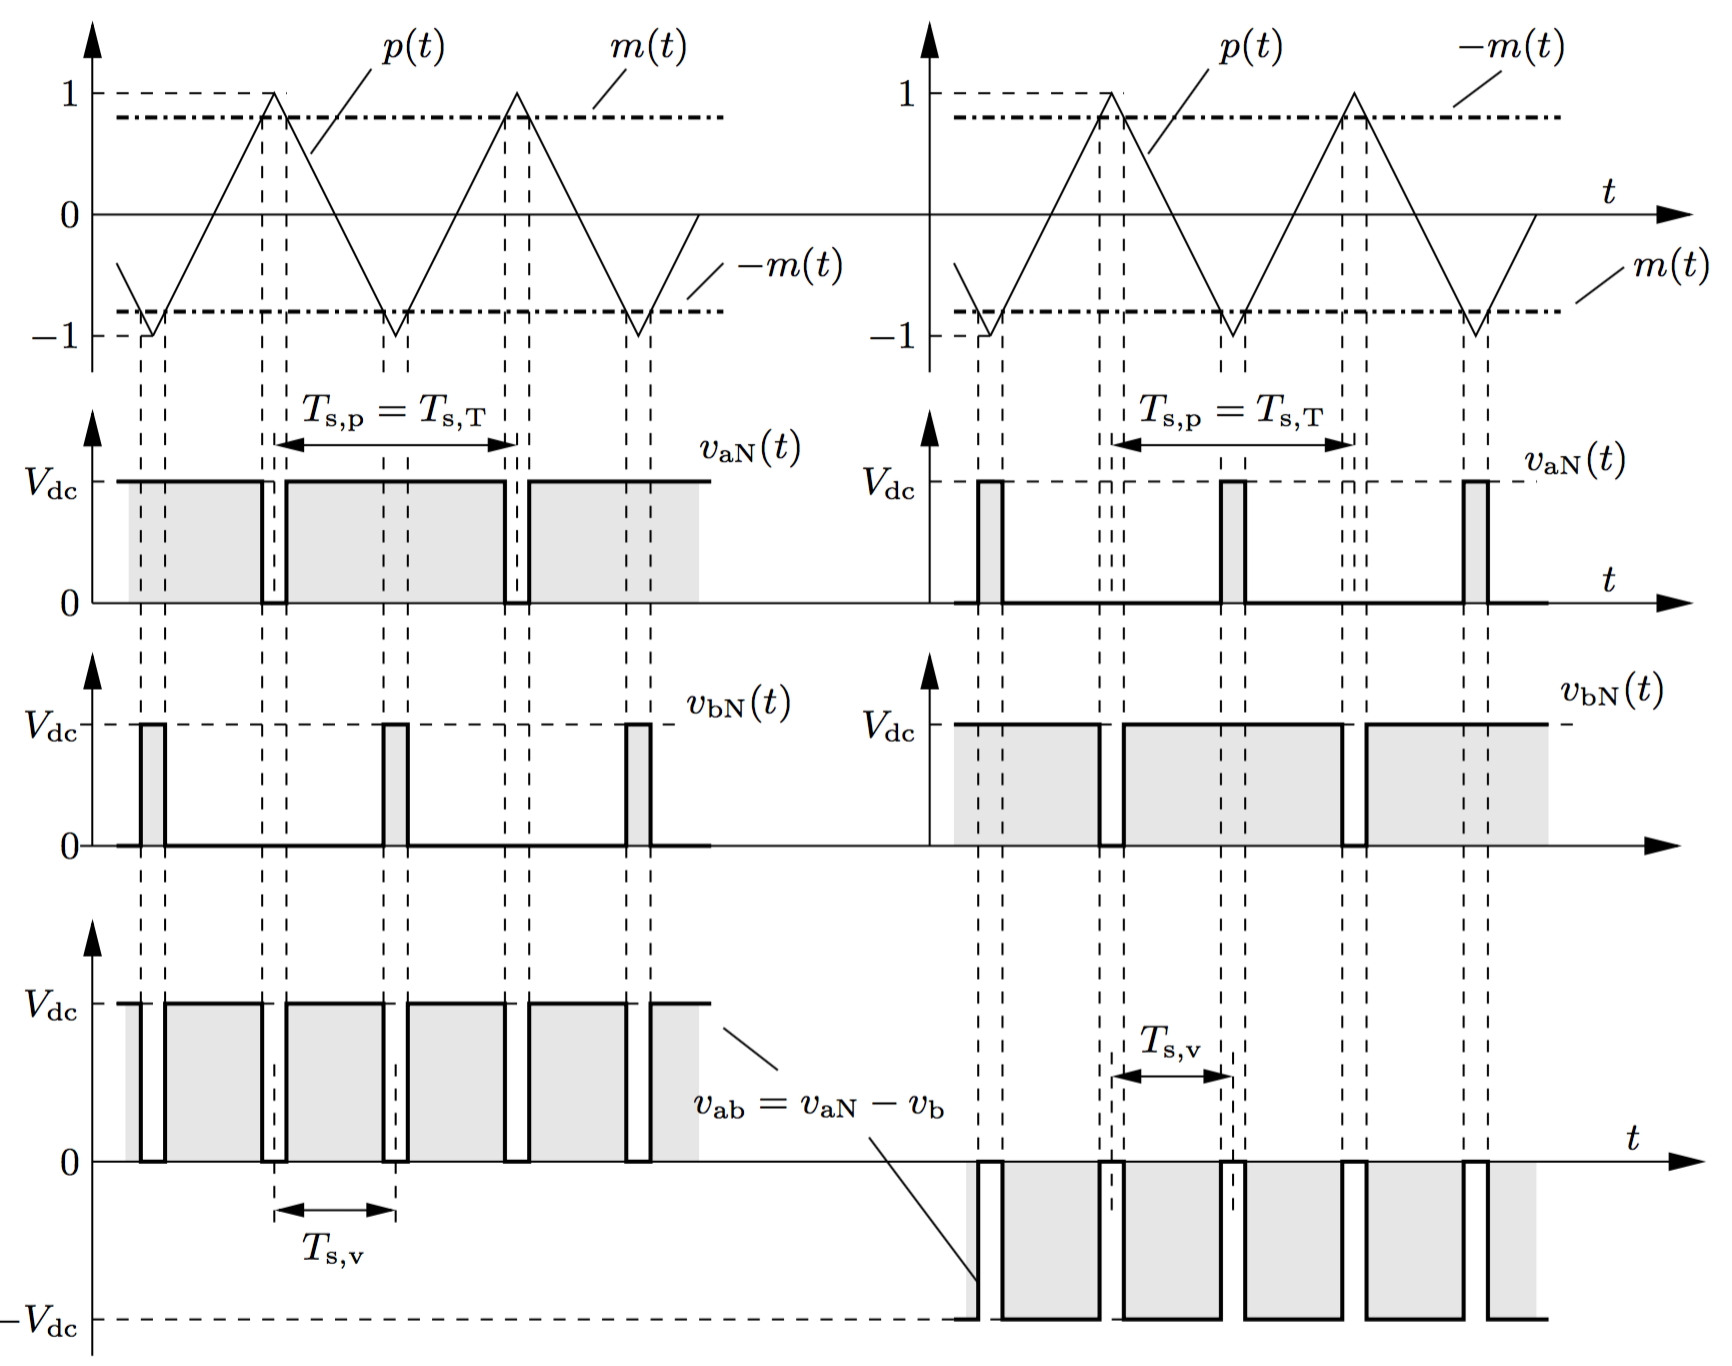
\includegraphics[scale=0.25]{ch4/11}
			\captionof{figure}{}
			\end{wrapfigure}
			On peut aussi utiliser 2 m(t) différentes pour les 2 bras. Le p(t) varie maintenant entre -1 et 1, avec une m(t) pour la commande du premier bras et -m(t) pour celle du second. Lorsque $m(t) > 0$, $v_{ab}(t)$ comprend 2 impulsions positives entre 0 et $V_{dc}$ par période de commutation. Il vient alors :
			\begin{equation}
				2 f_{s,p} = 2f_{s,T} = f_{s,v}.
			\end{equation}
			Remarquons les intervalles à sortie nulle, court-circuit de la charge. La tension de sortie est pareil que le précédent cas. \\
			
		\subsubsection{Comparaison des schémas bipolaire et unipolaire}
			\begin{wrapfigure}[8]{r}{6.5cm}
			\vspace{-5mm}
			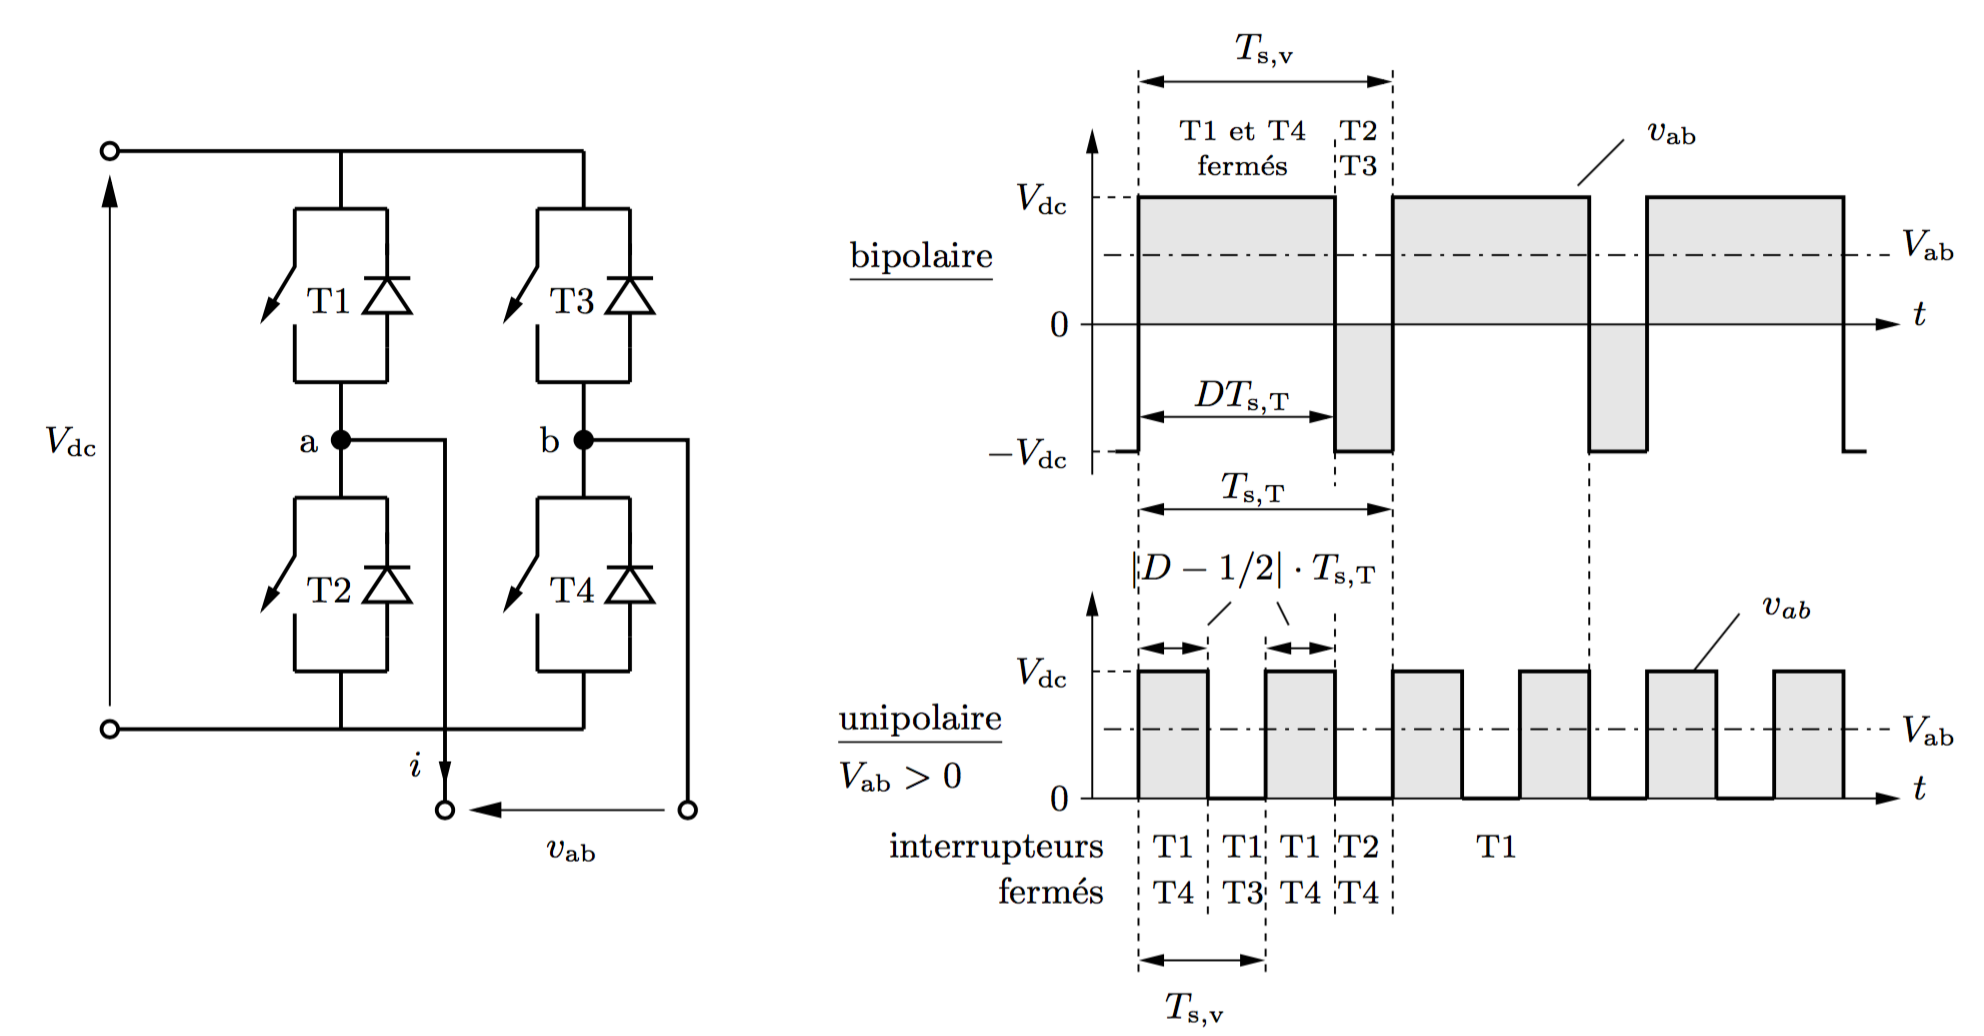
\includegraphics[scale=0.2]{ch4/12}
			\captionof{figure}{}
			\end{wrapfigure}
			Dans le cas bipolaire, on a par période de commutation, une impulsion positive de durée $DT_{s,T}$ et une impulsion négative de durée $(1-D)T_{s,T}$. Dans le cas unipolaire, par période de commutation on a 2 impulsions de même signe et de durée $|D-1/2|T_{s,T}$. L'écart entre les 2 cas est d'autant plus grand que D est proche de 0.5.
			\newpage
			
	\subsection{Couverture dans le plan tension-courant}
		\begin{wrapfigure}[10]{l}{7.5cm}
		\vspace{-5mm}
		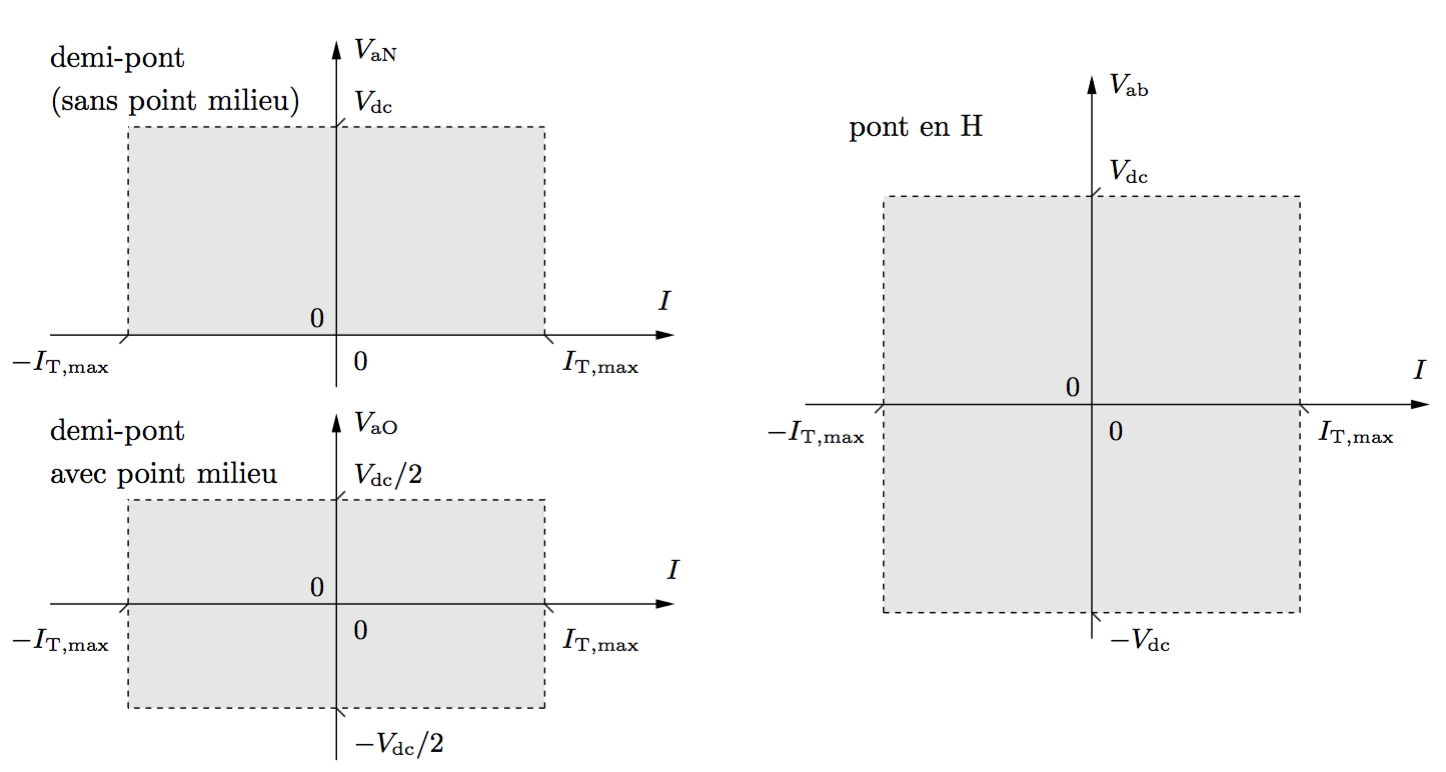
\includegraphics[scale=0.28]{ch4/13}
		\captionof{figure}{}
		\end{wrapfigure}
		Les \textbf{hacheurs} effectuent une conversion DC-DC entre $V_{dc}$ positive à l'entrée et une sortie moyenne positive ou négative $V_{aN}, V_{aO}$ ou $V_{ab}$. Pas de contrainte sur le signe de $i(t)$, mais sa valeur moyenne doit être limité : $-I_{T,min}\leq I \leq I_{T,max}$. En fonction du signe du courant par rapport à celle de la tension de sortie, la puissance s'écoule dans un sens. On distingue alors 4 quadrants dans le plan tension versus courant pour les hacheurs. 
		
	\subsection{Déformation du courant absorbé par une charge inductive}
		\begin{wrapfigure}[8]{r}{9cm}
		\vspace{-5mm}
		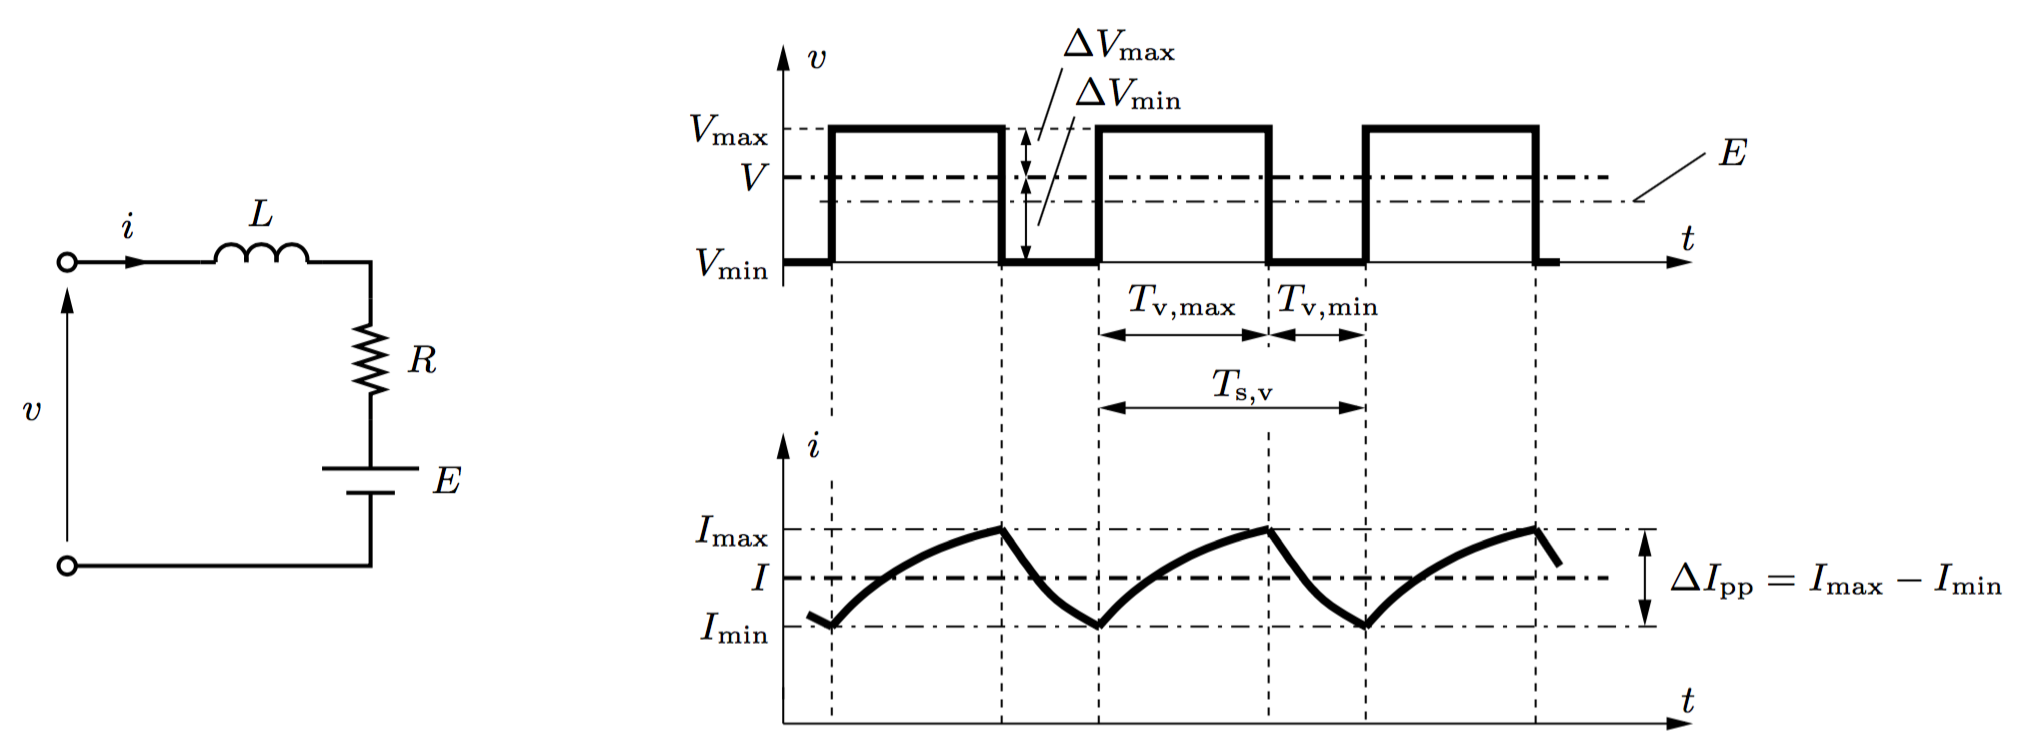
\includegraphics[scale=0.25]{ch4/14}
		\captionof{figure}{}
		\end{wrapfigure}
		Soit une charge RLE alimentée par une tension qui oscille entre $V_{min}$ et $V_{max}$, avec une période $T_{s,v}$ qui dépend de $f_{s,T}$ et du type de MLI. On considère le cas simplifié d'un régime établi et d'une tension $E=cst$. Les valeurs instantanées et moyennes sont reliées comme suit :\\
		\begin{equation}
			v(t) = Ri(t) + L\frac{di}{dt} + E \qquad et \qquad V = RI + E.
		\end{equation}
		
		En soustrayant ces deux équations, on trouve pour les variations :
		\begin{equation}
			\Delta v(t) = R\delta i(t) + L\frac{d\Delta i}{dt}.
		\end{equation}
		$\Delta v(t)$ est constant par morceau et vaut $\Delta V_{max}$ pendant un intervalle $T_{v,max}$ et $\Delta V_{min}$ pendant $T_{v,min}$, avec $T_{v,min} + T_{v,max} = T_{s,v}$. Comme la valeur moyenne de $\Delta v(t) = 0$, on a :
		\begin{equation}
			\Delta V_{max}T_{v,max} + \Delta V_{min}T_{v,min} = 0 \qquad avec \qquad \Delta V_{max} \geq 0 \ et \ \Delta V_{min} \leq 0
		\end{equation}
		$i(t)$ varie en dents de scie avec des flancs montants de durée $T_{v,max}$ et descendant $T_{v,min}$. Si la constante de temps $\tau = L/R \gg T_{s,v}$, la pente des flancs peut être vue constante et vaut soit $\Delta V_{max}/L$ soit $\Delta V_{min}/L$. L'ondulation crête à crête de $\Delta i(t)$ et $i(t)$ est donnée par :
		\begin{equation}
			\Delta I_{pp} = \frac{\Delta V_{max}T_{v,max}}{L} = -\frac{\Delta V_{min}T_{v,min}}{L}.
		\end{equation}
		
		L'augmentation de $I_{rms}$ en raison de l'ondulation donne lieu à :
		\begin{equation}
		\begin{array}{c}
			I_{rms} = \sqrt{I^2+(\Delta I_{rms})^2} \qquad avec \\
			\Delta I_{rms} = (\Delta i)_{rms} = \sqrt{\frac{1}{T_{s,v}}\int _{t_0}^{t0+T_{s,v}}(\Delta i)^2\, dt} = \Delta I_{pp} \sqrt{\int _{-1/2}^{1/2}x^2\, dx} 
		\end{array}
		\end{equation}
		Il vient finalement que :
		\begin{equation}
			\Delta I_{rms} = \frac{1}{2\sqrt{3}}\Delta I_{pp}.
		\end{equation}
		Les pertes Joules supplémentaires dans R de la charge sont $R(\Delta I_{rms})^2$. \\
		
		\textbf{Demi-pont sans point milieu à l'entrée} \qquad On a $T_{s,v} = T_{s,T}$, $V_{aN} = DV_{dc}, T_{v,max} = DT_s, \Delta V_{max} = V_{dc}-V_{aN}= (1-D)V_{dc}$ et il vient que :
		\begin{equation}
			\Delta I_{pp} = (1-D)D\frac{V_{dc}}{f_{s,T}L}= (1-D)\frac{V_{aN}}{f_{s,T}L}. 
		\end{equation}
		On peut donc diminuer l'ondulation en augmentant L et/ou $f_{s,T}$. Elle dépend aussi de D et est maximum pour D = 0.5. \\
		
		\textbf{Demi-pont avec point milieu à l'entrée} \qquad On a $T_{s,v} =T_{s,T}, V_{aO} = (2D-1)V_{dc}/2, T_{v,max}=DT_{s,T}, \Delta V_{max} = V_{dc}/2-V_{aO = (1-D)V_{dc}}$ et il vient :
		\begin{equation}
			\Delta I_{pp} = (1-D)D\frac{V_{dc}}{f_{s,T}L} = \frac{2(1-D)D}{2D-1}\frac{V_{aO}}{f_{s,T}L}.
		\end{equation}
		\ \\
		
		\textbf{Pont en H et schéma bipolaire}\qquad On a $T_{s,v} = T_{s,T}, V_{ab}=(2D-1)V_{dc}, T_{v,max}=DT_{s,T}, \Delta V_{max}= V_{dc}-V_{ab}=2(1-D)V_{dc}$ et :
		\begin{equation}
			\Delta I_{pp} = 2(1-D)D\frac{V_{dc}}{f_{s,T}L} = \frac{2(1-D)D}{2D-1}\frac{V_{ab}}{f_{s,T}L}.
		\end{equation}
		
		\ \\ \textbf{Pont en H et schéma unipolaire} \qquad On a en considérant une tension moyenne positive ($0.5\leq D\leq 1$) $T_{s,v} = T_{s,T}/2, V_{ab} =(2D-1)V_{dc}\geq 0, V_{max}=V_{dc}, T_{v,max}=(D-0.5)T_{s,T}, V_{min}=0, T_{v,min}= (1-D)T_{s,T}, \Delta V_{max}= V_{dc}-V_{ab}=2(1-D)V_{dc}$ et :
		\begin{equation}
			\Delta I_{pp} = (1-D)(2D-1)\frac{V_{dc}}{f_{s,T}L} = (1-D)\frac{V_{ab}}{f_{s,T}L}
		\end{equation}
		
		Pour une tension moyenne négative ($0\leq D\leq 0.5$) $T_{s,v} = T_{s,T}/2, V_{ab} =(2D-1)V_{dc}\leq 0, V_{max}=0, T_{v,max}=DT_{s,T}, V_{min}=-V_{dc}, T_{v,min}= (0.5-D)T_{s,T}, \Delta V_{max}= 0-V_{ab}=(1-2D)V_{dc}$ et :
		\begin{equation}
			\Delta I_{pp} = D(1-2D)\frac{V_{dc}}{f_{s,T}L} = D\frac{-V_{ab}}{f_{s,T}L}.
		\end{equation}
		Le schéma unipolaire donne lieu à un courant beaucoup moins ondulé que le cas bipolaire quand on s'éloigne des cas extrêmes D = 0 ou D=1. La différence est la plus grande quand D=0.5. Ces expressions restent valables dans le transitoire à condition de pouvoir scinder la variation fondamentale des grandeurs et celle qui est due aux commutations.
		
	\subsection{Temps mort}
		\begin{wrapfigure}[11]{l}{7cm}
		\vspace{-5mm}
		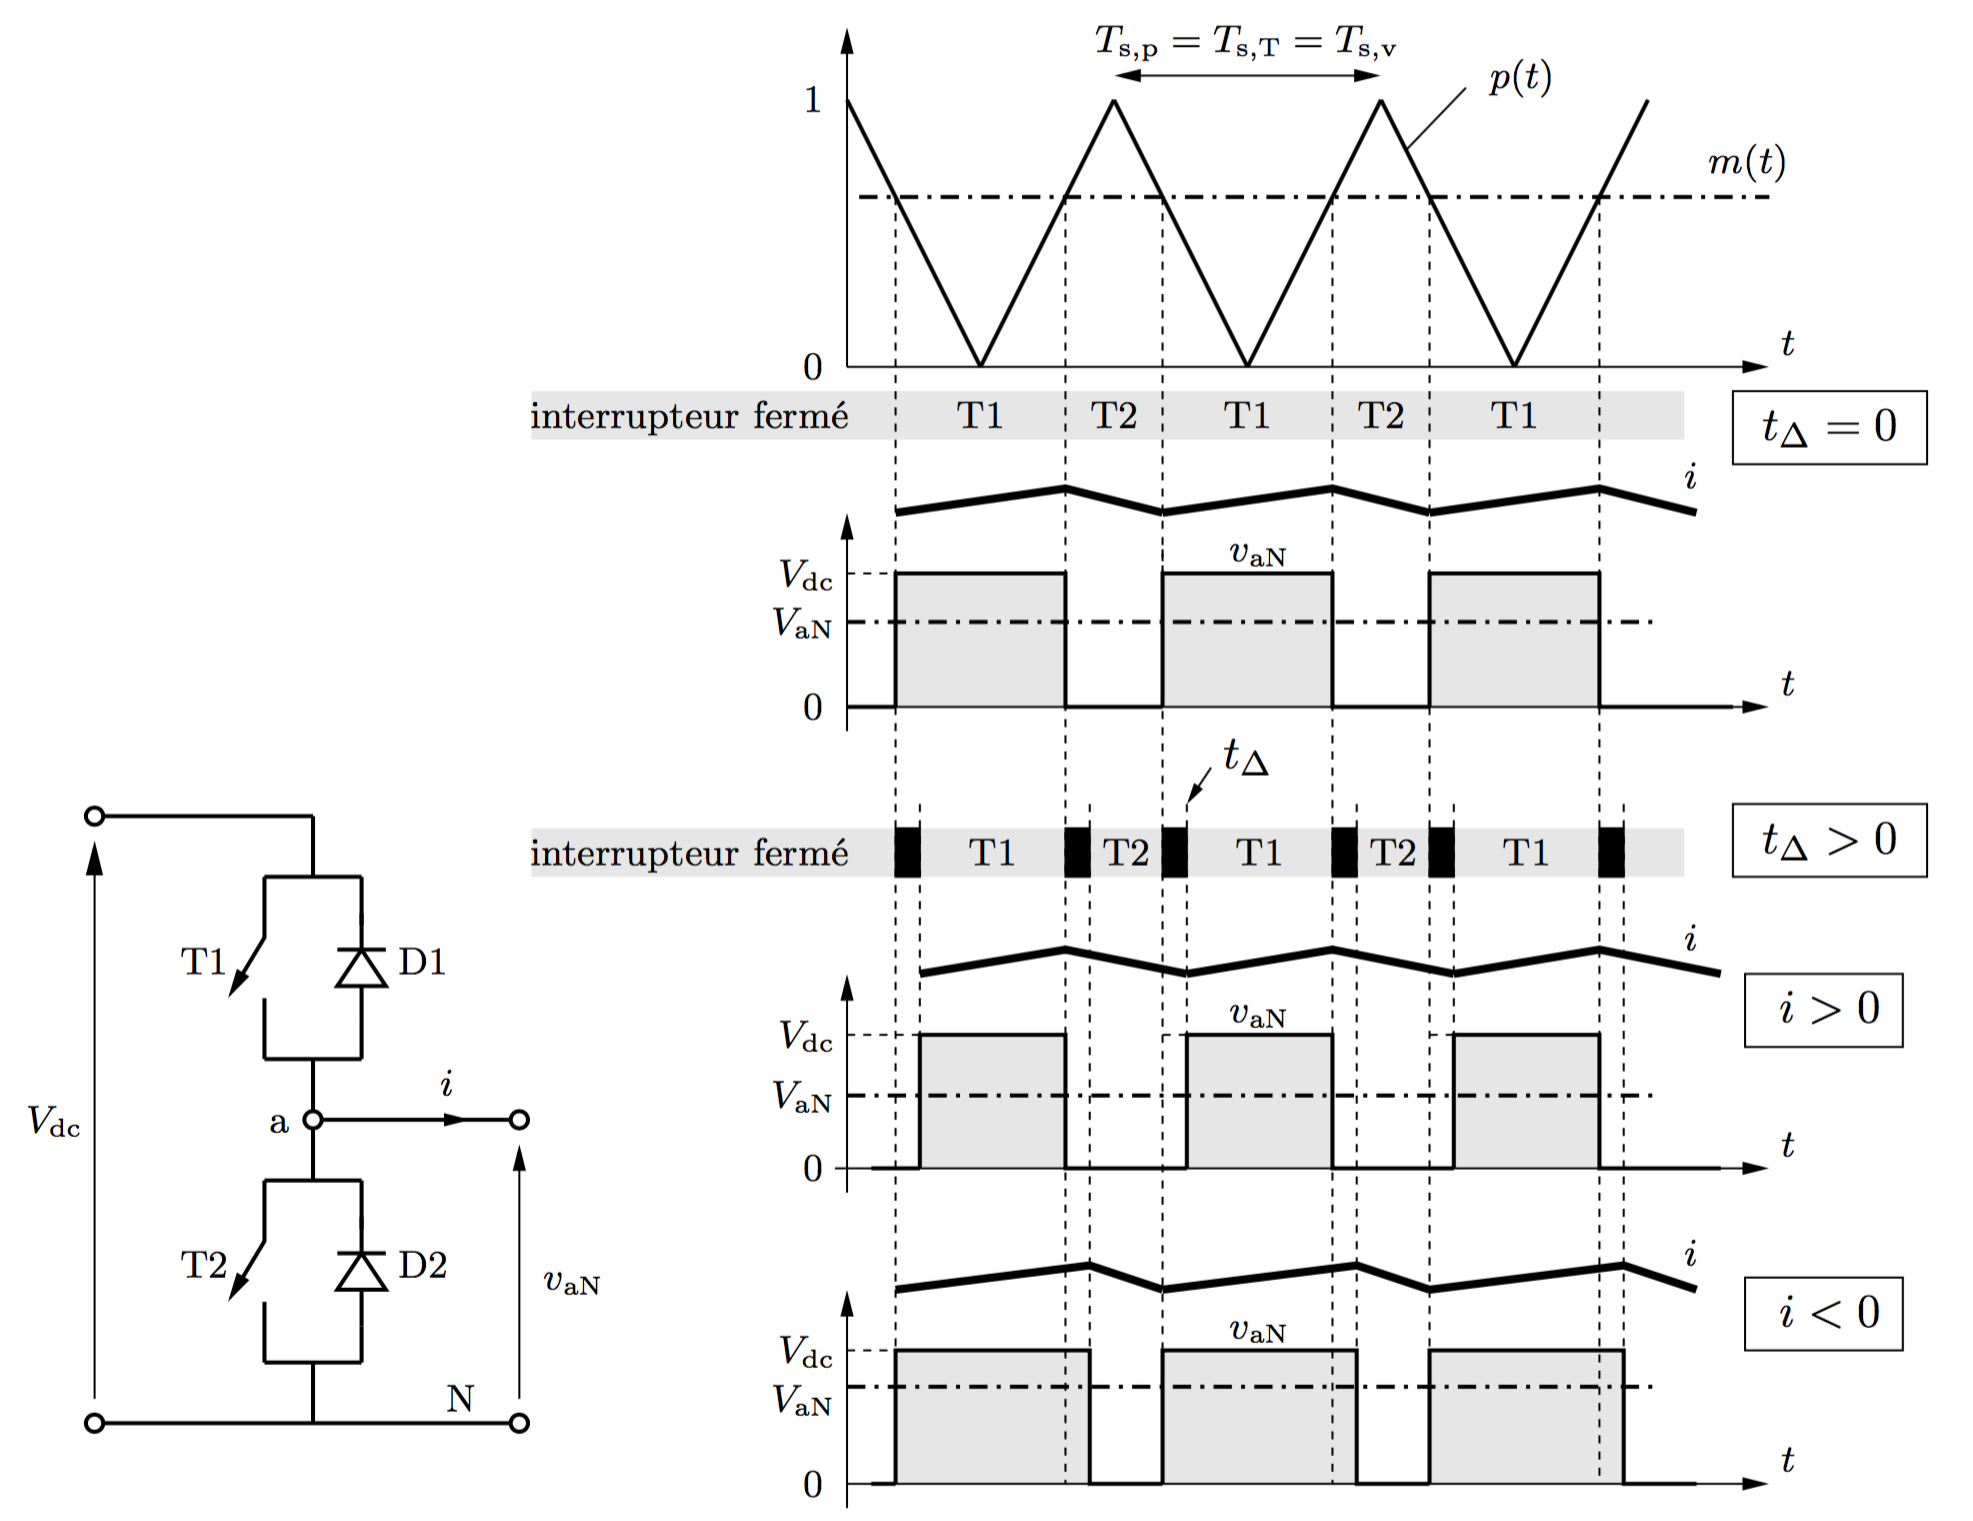
\includegraphics[scale=0.2]{ch4/15}
		\captionof{figure}{}
		\end{wrapfigure}
		Il faut dans la pratique intercaler un court intervalle durant lequel les 2 interrupteurs d'un bras sont ouverts pour éviter un court-circuit lors des commutations. Dans le cas d'un \textbf{demi-pont}, durant les courts instants où T1 et T2 sont ouverts en même temps, le sens de $i$ détermine la valeur de $v_{aN}$. S'il est >0, il circulera dans D2 et $v_{aN} =0$, si $i<0$, il circulera dans D1 et $v_{aN} = V_{dc}$. La figure ci-contre montre l'effet d'un report de la \textbf{fermeture} sur la tension de sortie, en supposant une charge inductive pour que $i$ faiblement ondulé ne s'inverse pas. 
		
\section{Onduleurs de tension monophasés}
	\begin{wrapfigure}[10]{l}{10cm}
	\vspace{-5mm}
	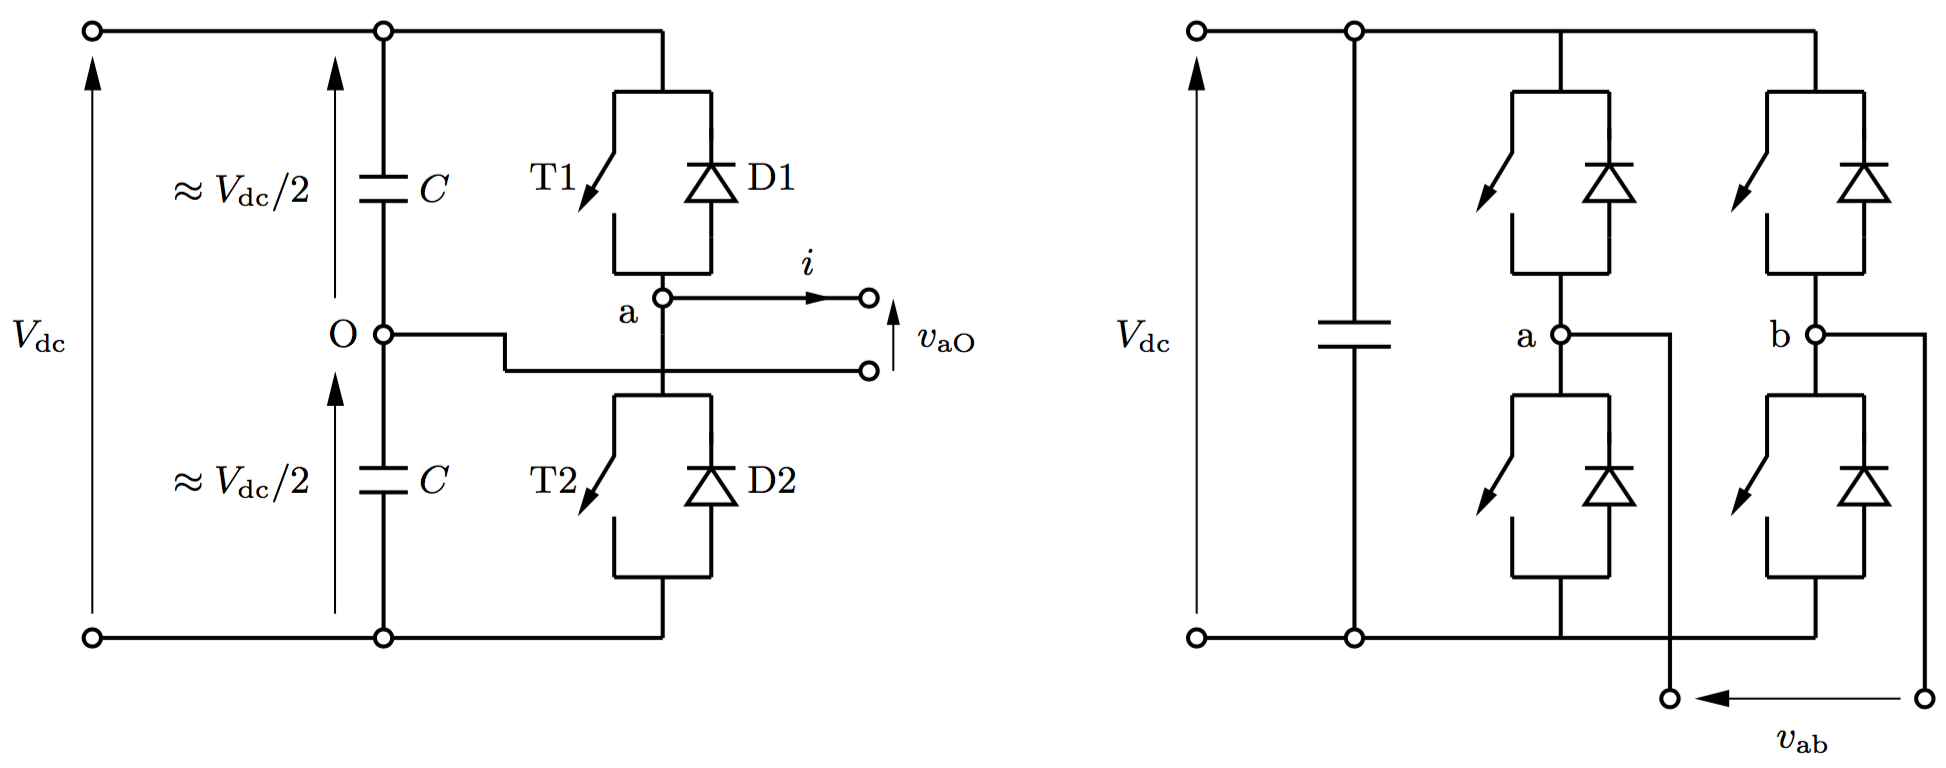
\includegraphics[scale=0.28]{ch4/16}
	\captionof{figure}{}
	\end{wrapfigure}
	Ils sont constitués de 1 ou 2 bras. Un demi-pont doit être muni d'un point milieu à la source. Au besoin on le crée à l'aide de 2 condensateurs de même C élevé.  Pour le pont en H c'est pas nécessaire. Dans la pratique, l'onduleur est alimenté par un redresseur, d'où le lissage par condensateur à l'entrée. Si la source est une batterie, le condensateur prend en charge la composante ondulatoire du courant et atténue l'effet de la résistance interne pendant que la batterie fournit la composante moyenne. 
	
	\subsection{MLI sinusoïdale linéaire}
		\subsubsection{Demi-pont}
			\begin{wrapfigure}[14]{r}{7cm}
			\vspace{-5mm}
			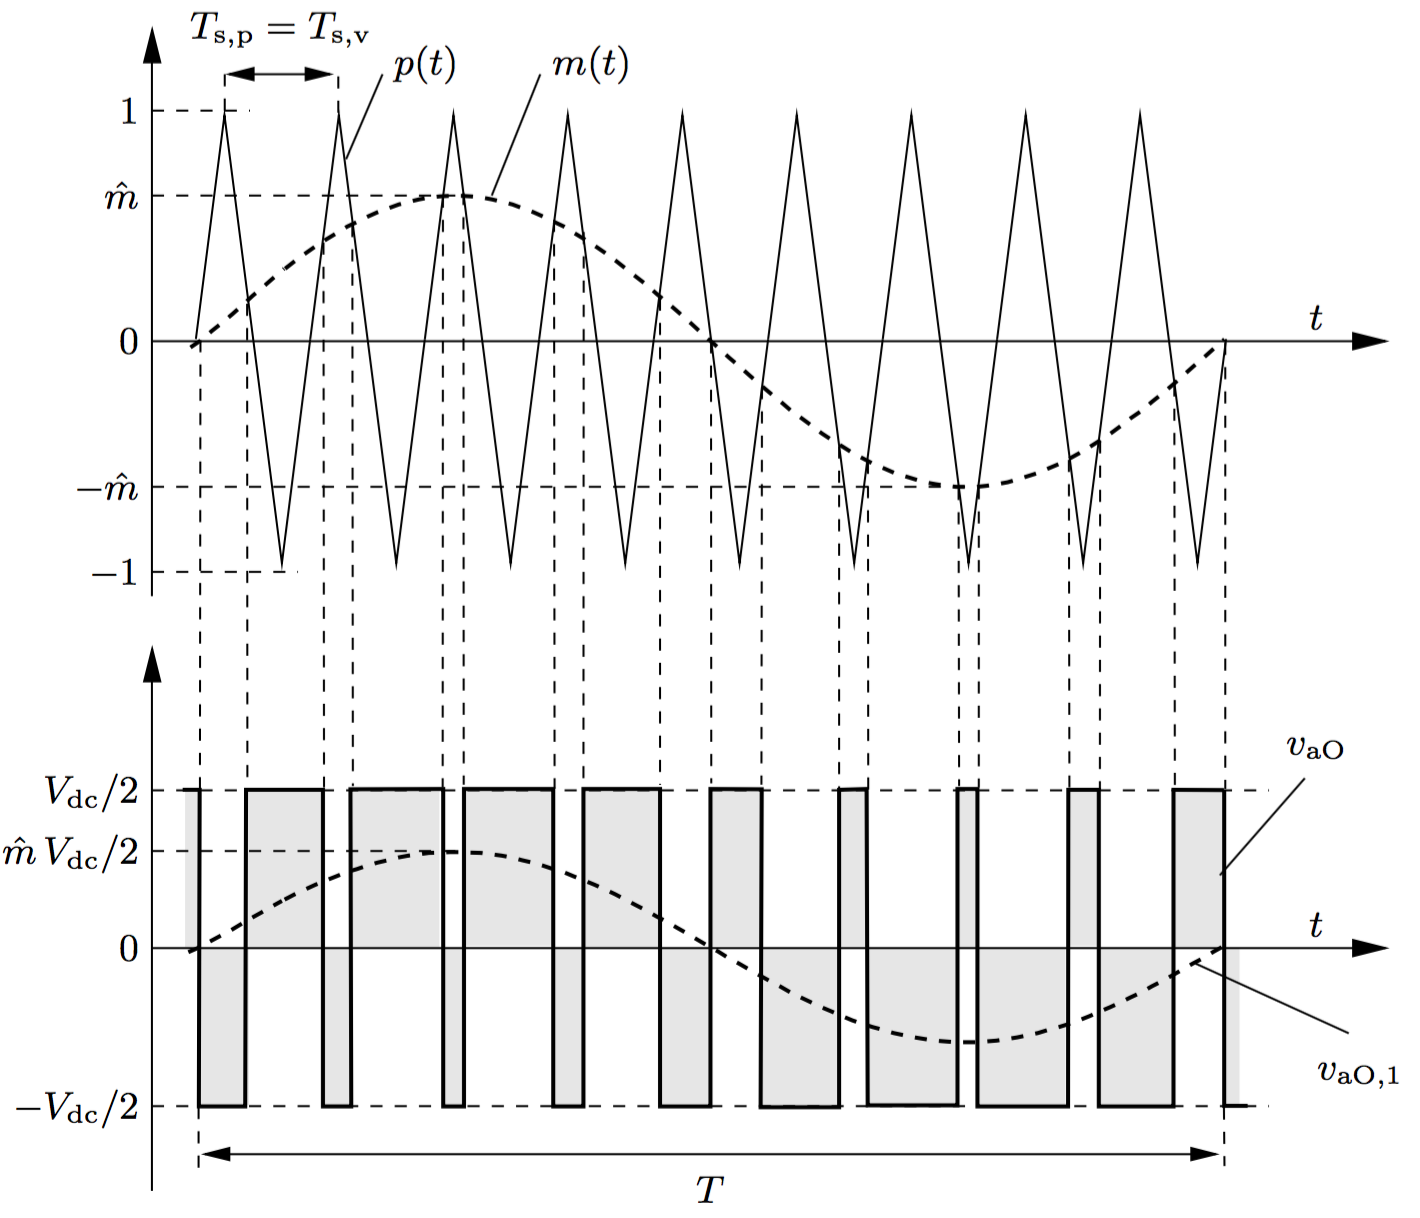
\includegraphics[scale=0.28]{ch4/17}
			\captionof{figure}{}
			\end{wrapfigure}
			On prend pour $p(t)$ un signal triangulaire de fréquence $f_{s,p}$ variant entre -1 et 1 et pour $m(t)$ une sinusoïde de fréquence $f$ et amplitude $\hat{m}$, image de la tension souhaitée. L'\textbf{angle de phase} constitue le 3e degré de liberté pour $m(t)$. On définit l'\textbf{indice d'amplitude} qui est le rapport des valeurs crêtes :
			\begin{equation}
				\hat{m} = \frac{\hat{m}}{1}
			\end{equation}
			Nous supposons dans un premier temps qu'il est $<1$. On définit également l'\textbf{indice de fréquence} : 
			\begin{equation}
				m_f = \frac{f_{s,p}}{f}.
			\end{equation}
			Il est de préférence \textbf{entier} (MLI synchrone) et dans le cas du demi-pont, impair. Avec $m_f$ entier et impair, $v_{aO}(t)$ possède la symétrie demi-onde $v_{aO}(t) = - v_{aO}(t+T/2)$, faisant disparaître les harmoniques paires. Lorsque $\hat{m}\leq 1$, m(t) et p(t) se croisent 2 fois par période de commutation $T_{s,T} = T_{s,p}$.\\
			
			 Si $m_f$ est suffisamment grand ($\geq 9$ par ex.) m(t) varie lentement comparé à p(t) et les discussions sur les hacheurs sont d'application. Il vient alors pour l'amplitude de la fondamentale $\hat{V}_{aO,1}$ : 
			 \begin{equation}
			 	\hat{V}_{aO,1} = \hat{m}\frac{V_{dc}}{2}.
			 \end{equation}
			 On parle alors de \textbf{modulation linéaire}. Outre la composante fondamentale de fréquence f, la tension comprend des harmoniques de fréquences élevées (pas de faible !) dont le rang impair s'écrit $h = km_f \pm l$ avec $k=1,2,...$ et $l$ entier et petit. 
			\newpage
			
		\subsubsection{Pont en H}
			\begin{wrapfigure}[16]{l}{5cm}
			\vspace{-5mm}
			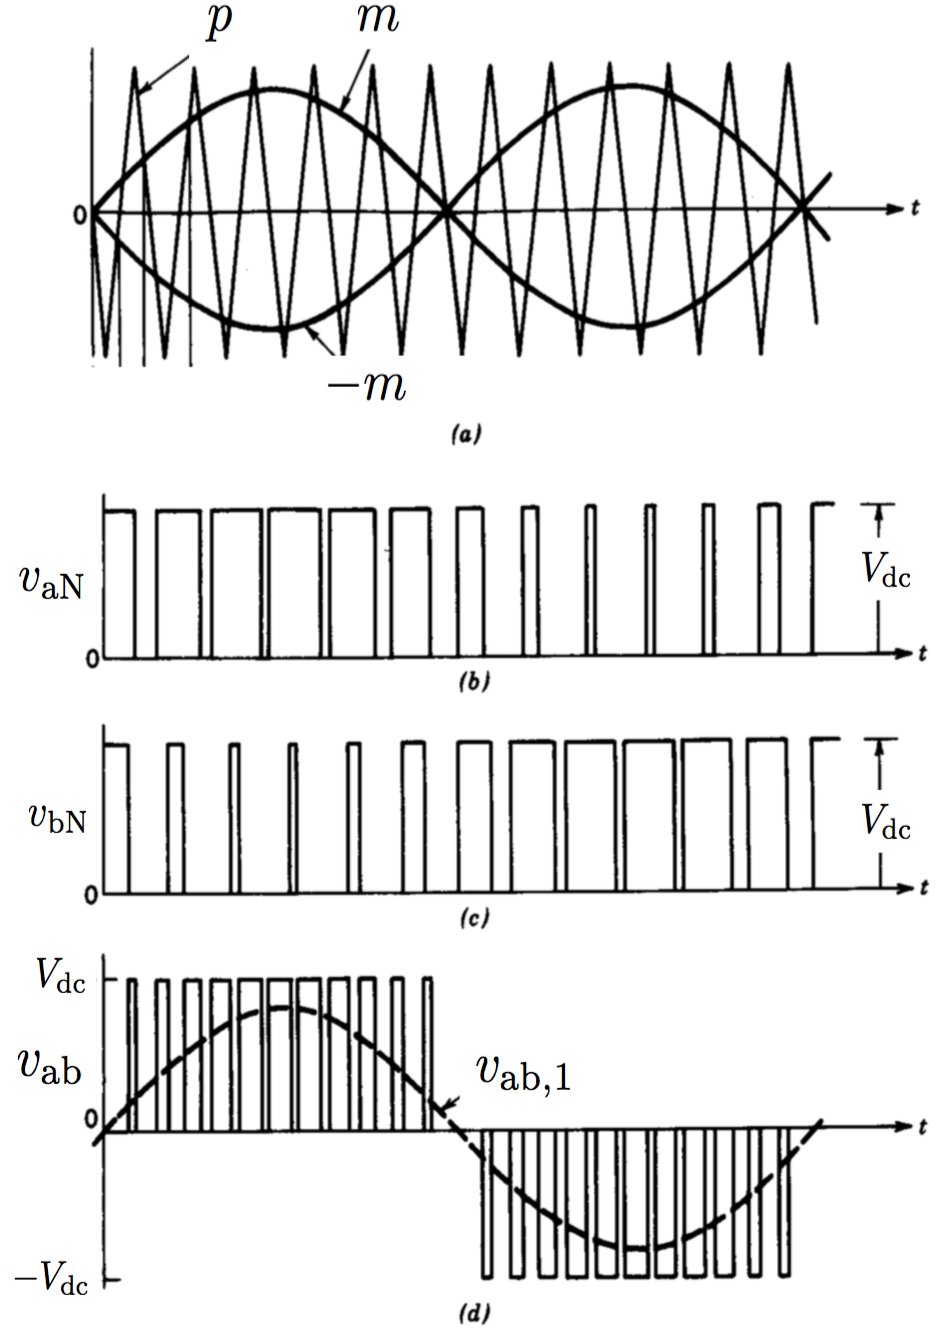
\includegraphics[scale=0.28]{ch4/18}
			\captionof{figure}{}
			\end{wrapfigure}
			On a de nouveau le cas bipolaire et unipolaire. Quel que soit le cas, on a pour la tension de sortie :
			\begin{equation}
				\hat{V}_{ab,1} = \hat{m}V_{dc}. 
			\end{equation}
			\textbf{MLI bipolaire} \qquad La forme d'onde obtenue est la même que celle pour le demi-pont sauf qu'elle varie de $-V_{dc}$ à $+V_{dc}$. Pour rappel, $m_{f}$ est de préférence entier et impair, conduisant à un spectre de tension de sortie très propre. 
			
			\paragraph{MLI unipolaire} \quad La figure ci-contre nous indique que les impulsions sont soit positives soir négatives (entre 0 et $\pm V_{dc}$) durant respectivement les alternances positives et négatives de $m(t)$. $m_f$ est maintenant entier et pair, auquel cas il possède la symétrie demi-onde. Les rangs d'harmonique sont donnés par $h=2km_f \pm l$. La fréquence de commutation a doublé $\Rightarrow$ bénéfique pour l'ondulation du courant avec L grand. 
			
	\subsection{Surmodulation et onde carrée}
\begin{center}
		\begin{minipage}{0.45\textwidth}
			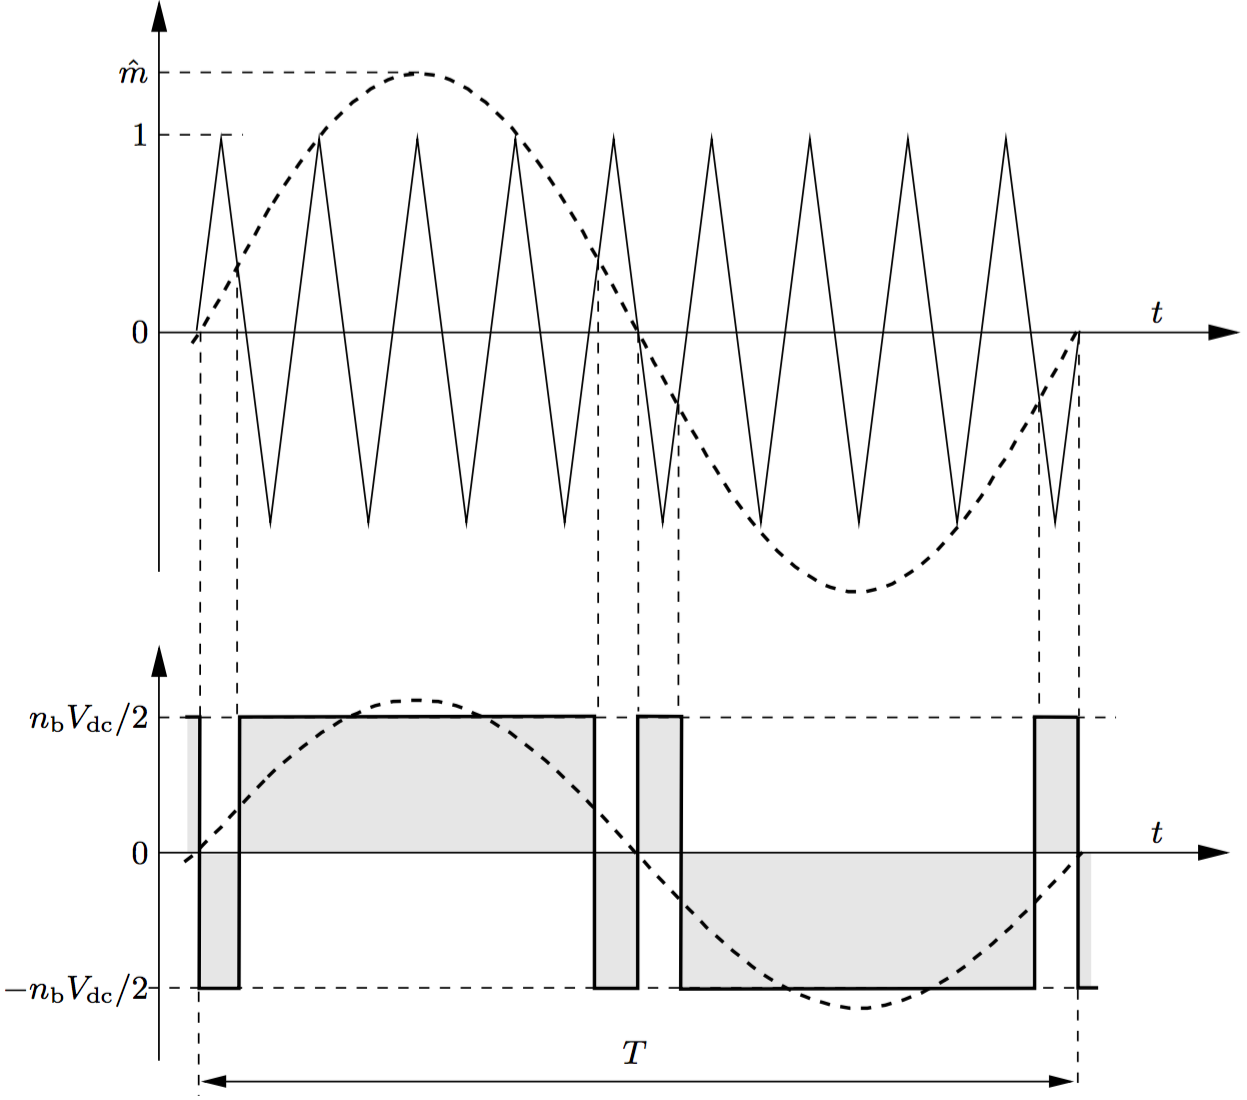
\includegraphics[scale=0.25]{ch4/19}
			\captionof{figure}{}
		\end{minipage}
		\begin{minipage}{0.45\textwidth}
			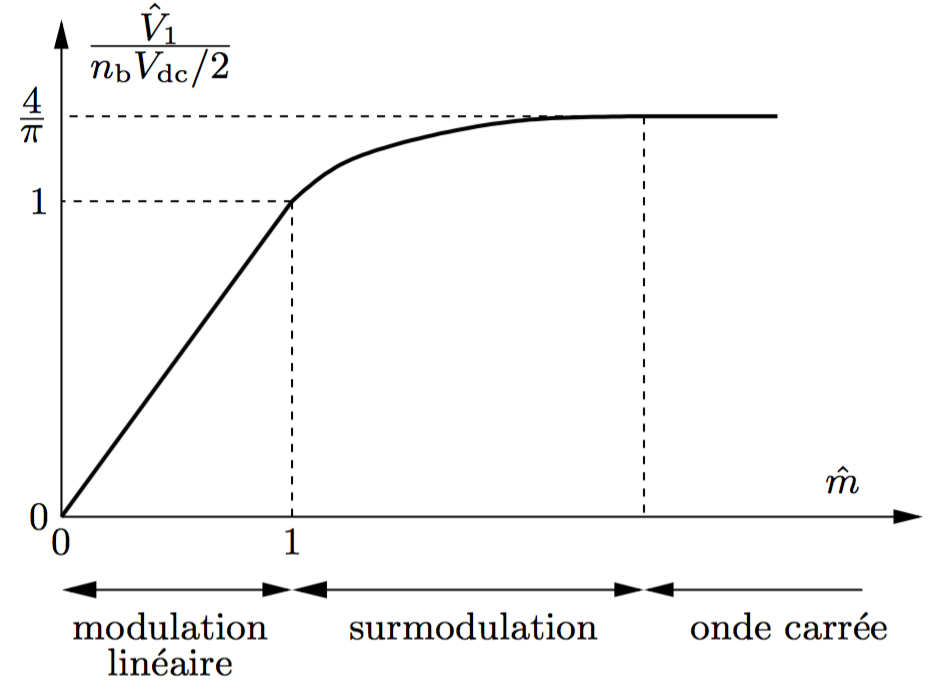
\includegraphics[scale=0.4]{ch4/20}
			\captionof{figure}{}
			\label{fig:4.18}
		\end{minipage}
\end{center}

		Correspond au cas $\hat{m}>1$. Il y a moins de commutations par période fondamentale T puisque p(t) et m(t) se croisent moins souvent, donc moins de pertes : $f < f_{s,T} < f_{s,p}$. Sur la figure on peut voir que l'amplitude du signal n'augmente plus de manière linéaire avec $\hat{m}$ et les harmoniques de faible rang apparaissent. 
		
		\paragraph{L'onde carrée}\quad A partir d'un certain $\hat{m}$ qui dépend de $m_f$ (entier), le croisement ne s'effectue que lors du passage par 0 de m(t) et on obtient une onde carrée dont l'amplitude du fondamentale de tension est maximum (\autoref{fig:4.18}):
		\begin{equation}
			\hat{V}_{1} = n_b \frac{4}{\pi}\frac{V_{dc}}{2}. 
		\end{equation}		  
		où $n_b = 1$ ou 2 selon qu'on est dans un demi-pont ou un pont en H bipolaire. Chaque interrupteur est ouvert fermé une seule fois par T. La $f_{s,T} = f$ est minimale, permettant l'utilisation des interrupteurs lents tels les GTO (pertes minimales). $V_1$ est max dans ce cas, mais doit être réglé via $V_{dc}$, donc nécessite la présence d'un \textbf{redresseur commandé} en amont à la place d'un redresseur à diode bon marché. Les harmoniques de faible rang sont un autre problème. \\
		
		La MLI linéaire requiert des interrupteurs plus rapides, ce plus $m_f$ est grand et occasionne plus de pertes de commutation. Par contre, on peut faire varier $\hat{V}_1$ par simple action sur $\hat{m}$. Les harmoniques étant de rang plus élevé, les harmoniques de courant sont de faible amplitude (si charge inductive). 
		
	\subsection{Charge RLE générique et composantes fondamentales et harmoniques du courant}
		\begin{wrapfigure}[8]{l}{7.5cm}
			\vspace{-5mm}
			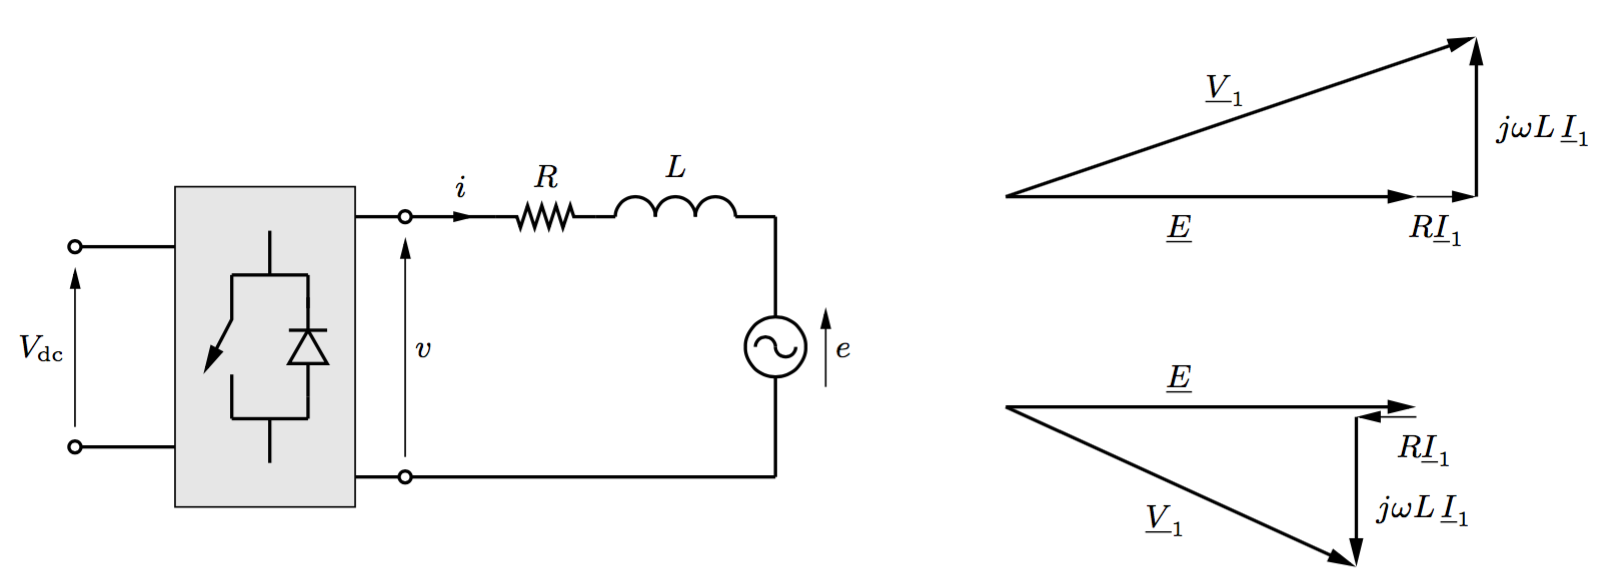
\includegraphics[scale=0.25]{ch4/21}
			\captionof{figure}{}
			\end{wrapfigure}
			On considère une charge RLE avec cette fois une source de f.e.m. $e(t) = \sqrt{2}E\cos (\omega t + \gamma _e)$. Il peut aussi s'agir d'un réseau monophasé et son équivalent de Thévenin. Dans la pratique, $R\ll X = \omega L$ (réactance) à la pulsation fondamentale et la déformation de $e(t)$ est négligée. Il est essentiel d'avoir la même pulsation pour $e(t)$ et le fondamental de la tension de sortie $v_1(t) = \sqrt{2}V_1 \cos (\omega t +\gamma _{v,1})$. En régime établi, $i_1(t)$ dans la charge est également à la même pulsation $\omega$. On peut représenter ces 3 grandeurs par les phaseurs reliés de la sorte :
			\begin{equation}
				\underline{E} = Ee^{j\gamma _e}, \underline{V}_1 = V_1e^{j\gamma _{v,1}}, \underline{I}_1 = I_1e^{j\gamma _{i,1}} \qquad \underline{V}_1=\underline{E}+(R+j\omega L)\underline{I}_1
			\end{equation}
			Ou encore en isolant le courant :
			\begin{equation}
				\underline{I}_1 = \frac{\underline{V}_1-\underline{E}}{R+j\omega L}.
			\end{equation}
			On voit qu'en agissant sur l'angle de phase et l'amplitude de $v_1(t)$, on peut commander $i_{1}(t)$ et ainsi le flux de puissance active te réactive. Sur la figure ci-contre, 2 cas particuliers selon que $\underline{I}_1$ est soir en phase soit en opposition de phase avec $\underline{E}$. Le circuit se comportera respectivement comme une charge et comme une source. 
			
			\paragraph{Harmoniques de courant} \quad Puisque pour $h>1$, $\underline{E}_h =0$, on a pour les valeurs efficaces des harmoniques $\underline{I}_h$ : 
			\begin{equation}
				\underline{I}_h = \frac{\underline{V}_h}{\sqrt{R^2+(h\omega L)^2}} \approx \frac{\underline{V}_h}{h\omega L}. 
			\end{equation}
			On voit donc que l'atténuation par l'inductance s'améliore avec le rang et leur pulsation $h\omega$ élevés. Les faibles rangs (h=3, 5, ...) sont relativement peu atténués. 
			
\section{Onduleurs de tension triphasés}
	\subsection{MLI sinusoïdale linéaire}
		\begin{wrapfigure}[7]{r}{5.5cm}
		\vspace{-5mm}
		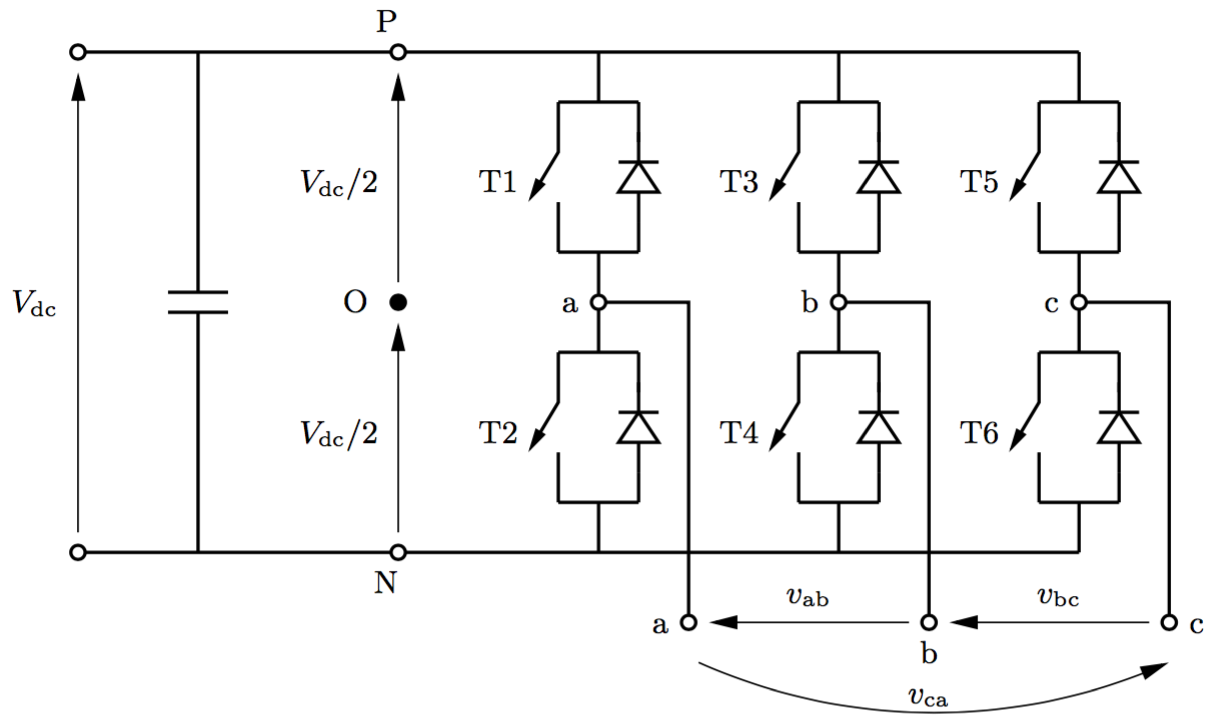
\includegraphics[scale=0.25]{ch4/22}
		\captionof{figure}{}
		\end{wrapfigure}
		On a cette fois 3 bras et la charge est raccordée aux 3 points milieux a, b et c. Le point milieu O du bus DC sert à la mise en équation, mais n'est pas indispensable au fonctionnement pratique de l'onduleur. Pour le cas linéaire, la commande des 6 interrupteurs peut se faire en comparant une $-1< p(t)<1$ de fréquence $f_{s,p}$ à 3 m(t) constituant un système triphasé équilibré, de même fréquence $f$, amplitude $\hat{m}_a=\hat{m}_b=\hat{m}_c$ et 
		
		\begin{wrapfigure}[11]{l}{4cm}
		\vspace{-5mm}
		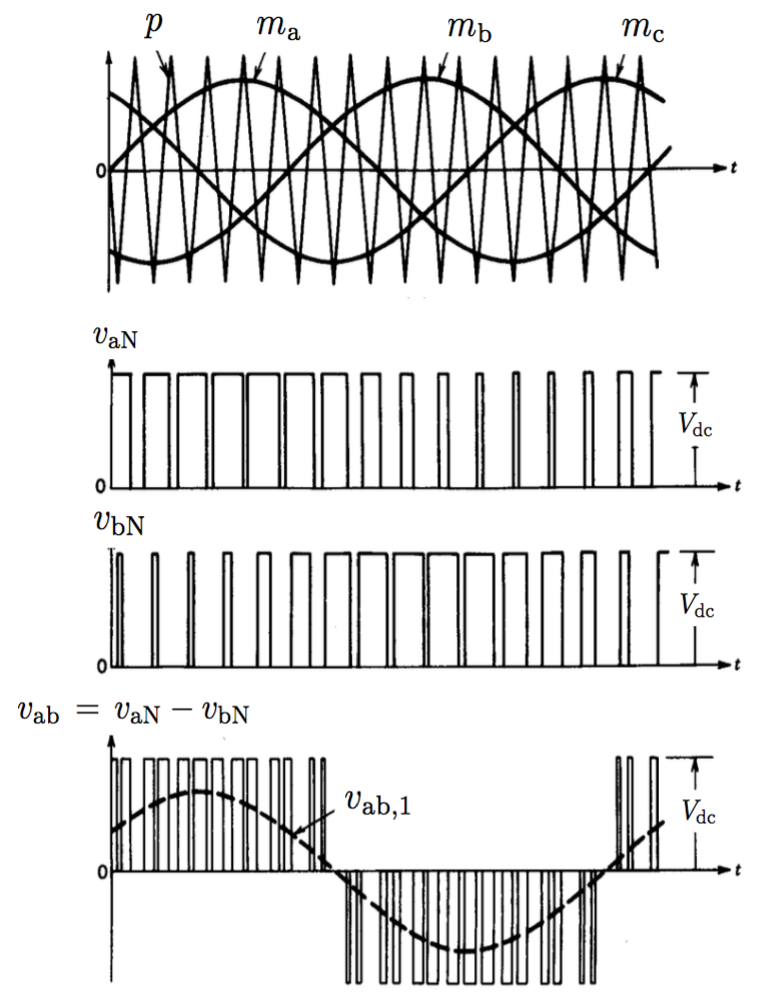
\includegraphics[scale=0.25]{ch4/23}
		\captionof{figure}{}
		\end{wrapfigure}
		déphasées de 120\degres . p(t) de valeur normalisée fait que \textbf{l'indice d'amplitude} est :
		\begin{equation}
			\hat{m} = \hat{m}_a = \hat{m}_b = \hat{m}_c \qquad \mbox{linéaire si } \hat{m} \leq 1.
		\end{equation}
		Pour des raisons de symétrie, il convient que l'i\textbf{ndice de fréquence} soit un multiple entier impair de 3. Si c'est le cas, les différents ensembles de tensions triphasés constituent des systèmes triphasés équilibrés. Il vient pour la composante fondamentale des tensions $v_{xO} = v_{xN}-V_{dc}/2$, avec $x \in \{a, b, c\}$ : 
		\begin{equation}
			\hat{V}_{xO,1} = \hat{m}\frac{1}{2}V_{dc}\qquad et \qquad V_{xO,1} = \hat{m}\frac{1}{2\sqrt{2}}V_{dc}
		\end{equation}
		
		Et pour la tension phase-phase avec un déphasage de 120\degres (p.ex. $v_{ab}(t) = v_{aO}(t) - v_{bO}(t)$) :
		\begin{equation}
			\hat{U}_{1} = \hat{m}\frac{\sqrt{3}}{2}V_{dc}\qquad et \qquad U_{1} = \hat{m}\frac{\sqrt{3}}{2\sqrt{2}}V_{dc}
		\end{equation}
		On remarque sur la figure que les tensions phase-phase sont unipolaires avec $m_f$ impulsions positive/négative par alternance positive/négative du fondamental de tension. Les harmoniques sont concentrés autour des fréquences multiples de $f_{s,p} =f_{s,T}$. Symétrie demi-onde $\Rightarrow$ pas de rang pair et la symétrie triphasée avec $v_{ab} + v_{bc} + v_{ca} = 0$, les rangs multiples de 3 sont absents dans les tensions phase-phase (absence de rang faible primordiale). 
		
	\subsection{Surmodulation et onde carrée}
		Pareil qu'en monophasé, quand $\hat{m}>1$ $v_1(t)$ augmente de manière non linéaire, $f_{s,T}$ est moindre et donc les pertes réduites. L'introduction d'harmoniques de faible rang est l'inconvénient majeur, mais celles de rang pair et multiple de 3 restent absentes. La précédente caractéristique reste valable et :
		\begin{equation}
			\hat{U}_1 = \frac{4}{\pi}\frac{\sqrt{3}}{2}V_{dc}\qquad et \qquad U_1 = \frac{\sqrt{6}}{\pi}V_{dc}.
		\end{equation}
		sont maximums.
		
	\subsection{Charge RLE générique et tensions phase-neutre}
	\begin{wrapfigure}[11]{r}{5.2cm}
	\vspace{-5mm}
	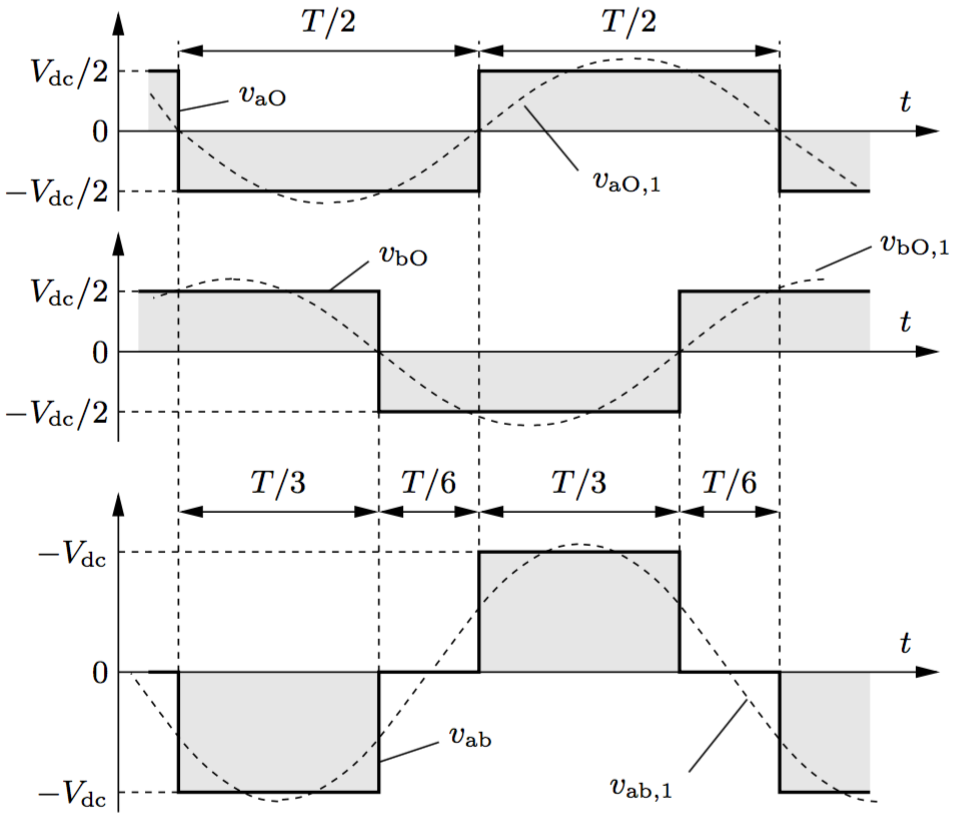
\includegraphics[scale=0.3]{ch4/28}
	\captionof{figure}{}
	\label{fig:4.22}
	\end{wrapfigure}
	On considère une charge symétrique avec connexion en étoile de point neutre $n$ régie par les 3 équations :
	\begin{equation}
		v_{xn} = Ri_x + L\frac{di_x}{dt} +e_x \qquad x\in \{ a, b, c \} .
	\end{equation}			
	Selon l'application et la finesse de la modélisation, les f.e.m. sont parfaitement sinusoïdale ou ont une certaine déformation. Nos 3 équations dépendent de l'onduleur triphasé ($V_{dc}$ + commande des interrupteurs).
	
	 \ \\ La somme des 3 courants de ligne est nulle. Supposons que la somme des $e_x$ est également nulle (souvent le cas dans la pratique). Par les équations précédentes on vérifie que :
	 \begin{equation}
	 	v_{an} +v_{bn}+v_{cn} = 0
	 	\label{eq:4.38}
	 \end{equation}
	 
	 On a ensuite la relation : 
	 \begin{equation}
	 	v_{xn} = v_{xN} - v_{nN}
	 	\label{eq:4.39}
	 \end{equation}
	 
	 \begin{wrapfigure}[12]{l}{6cm}
		\vspace{-5mm}
		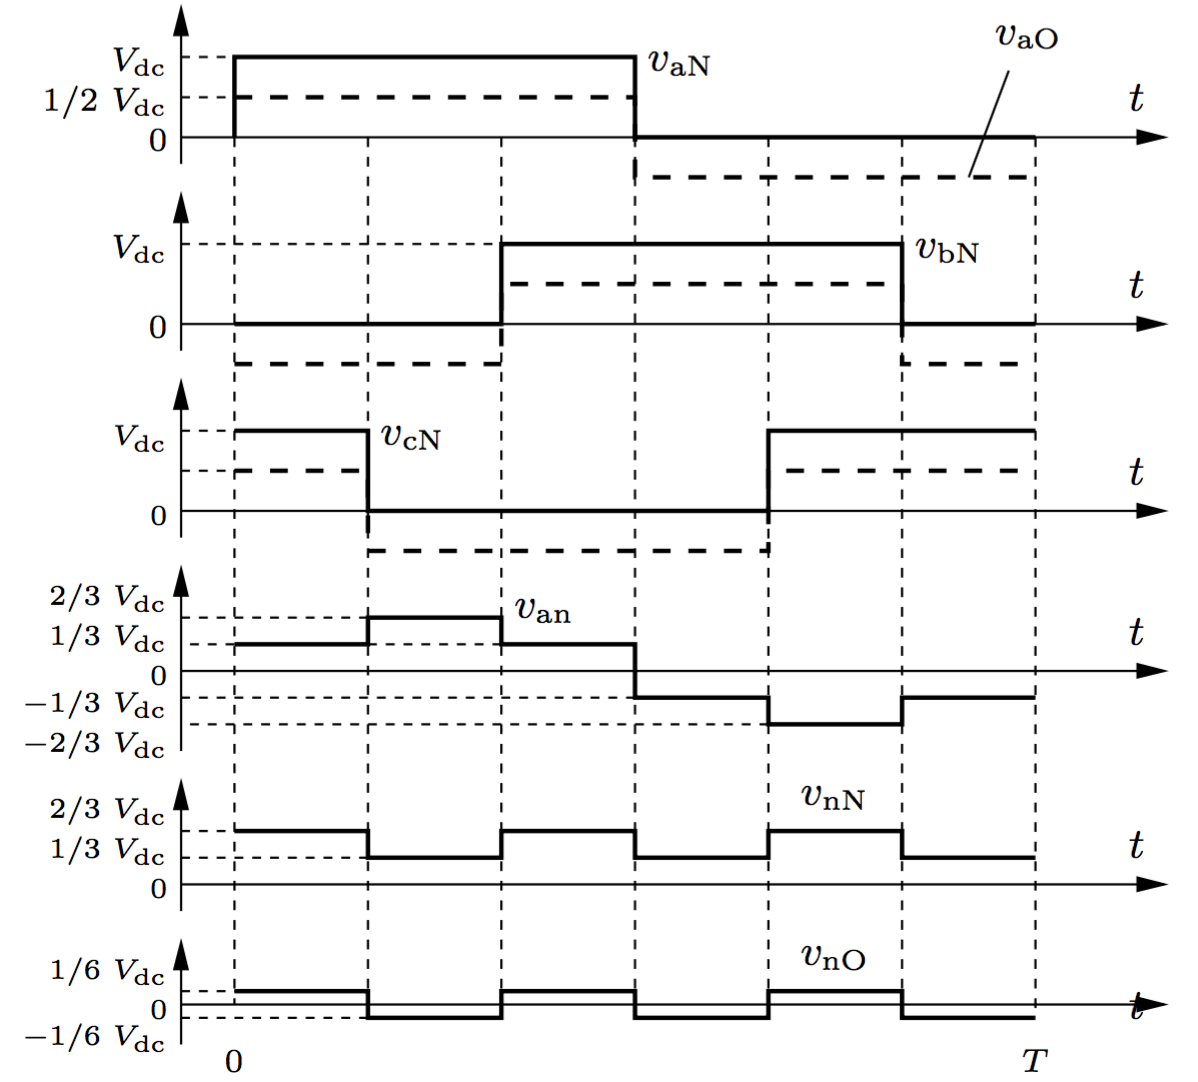
\includegraphics[scale=0.28]{ch4/24}
		\captionof{figure}{}
		\end{wrapfigure}
		où $v_{xN}$ vaut soit 0 soit $V_{dc}$, suivant la commande du bras x, en négligeant le temps mort et supposant que les semi-conducteurs sont idéaux. On peut aussi avoir, en considérant le point milieu :
	 \begin{equation}
	 	v_{xn} = v_{xO} - v_{nO}
	\end{equation}	  
	$où v_{x0}$ vaut soit $-V_{dc}/2$ soit $+V_{dc}/2$. En utilisant \eqref{eq:4.38}, on trouve :
	\begin{equation}
	\begin{aligned}
	v_{nN} &= \frac{1}{3} (v_{aN} +v_{bN}+v_{cN})\\
	v_{nO} &= \frac{1}{3} (v_{aO} +v_{bO}+v_{cO})
	\end{aligned}
	\end{equation}
	En remplaçant dans \eqref{eq:4.39} on obtient : 
	\begin{equation}
	\begin{aligned}
	v_{an} &= \frac{1}{3} (2v_{aN} -v_{bN}-v_{cN})\\
	v_{bn} &= \frac{1}{3} (2v_{bN} -v_{aN}-v_{cN})\\
	v_{cn} &= \frac{1}{3} (2v_{cN} -v_{bN}-v_{aN})
	\end{aligned}	
	\end{equation}
	Et similairement pour O. Tout ceci est illustré dans le cas d'une commutation en onde carrée ci-contre. On remarque que les $v_x$ prennent les valeurs discrètes $\pm \frac{1}{3}V_{dc}$ et $\pm \frac{2}{3}V_{dc}$, $v_{nN}$ prend 2 valeurs $ \frac{1}{3}V_{dc}$ et $\frac{2}{3}V_{dc}$ et sa moyenne vaut $V_{dc}/2$; et finalement $v_{aO}=\pm \frac{1}{6}V_{dc}$ qui est purement AC de fréquence $3f$. Le cas d'une MLI linéaire est présenté sur la figure ci-bas, on y remarque en plus des intervalles de tension nulle, entraînant une composante fondamentale moins élevée. 
	
	\begin{center}
		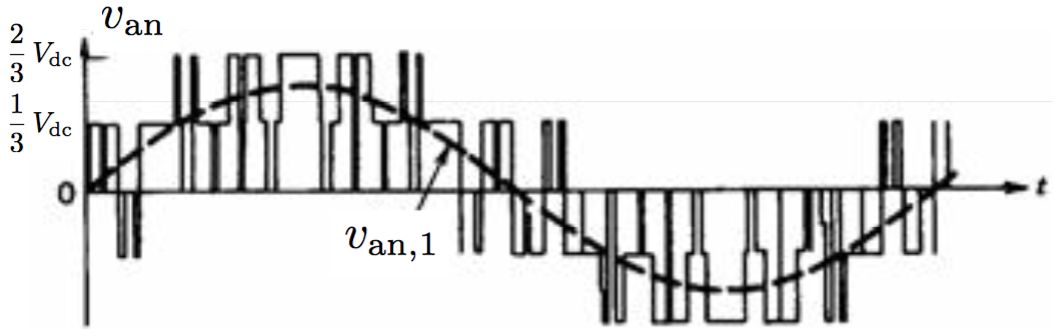
\includegraphics[scale=0.5]{ch4/25}
		\captionof{figure}{}
	\end{center}
	
	\subsection{Modulation à vecteur spatial}
		\paragraph{Régime quelconque}\quad Définissons le vecteur spatial $\vec{v}(t)$ des 3 tensions phase-neutre $v_{an}(t), v_{bn}(t)$ et $v_{cn}(t)$ comme le nombre complexe : 
		\begin{equation}
			\vec{v}(t) = \frac{2}{3} \left( v_{an}(t) + e^{j2\pi/3}v_{bn}(t)+ e^{-j2\pi/3}v_{cn}(t) \right),
		\end{equation}
		supposant l'ordre de phase direct $a\rightarrow b \rightarrow c$. Les parties réelle et imaginaire $\alpha$ et $\beta$ sont :
		\begin{equation}
			v_{\alpha}(t) = \frac{2}{3} v_{an}(t) - \frac{1}{3}(v_{bn}(t) + v_{cn}(t)) \qquad et \qquad v_{\beta}(t) = \frac{\sqrt{3}}{3}(v_{bn}(t) - v_{cn}(t)).
			\label{eq:4.44}
		\end{equation}
		Le point neutre n peut en fait être remplacé par un point m quelconque puisque :
		\begin{equation}
			\vec{v}(t) = \frac{2}{3} \left( v_{am}(t) + e^{j2\pi/3}v_{bm}(t)+ e^{-j2\pi/3}v_{cm}(t) \right) + \frac{2}{3}v_{nm}(t) \underbrace{\left( 1+e^{j2\pi/3} + e^{-j2\pi/3}\right)}_{=0}. 
		\end{equation}
		On peut exprimer \eqref{eq:4.44} en tension phase-phase en se rappelant que leur somme est nulle : 
		\begin{equation}
			v_\alpha (t) = \frac{2}{3}(v_{ab}(t) - v_{ca}(t)) \qquad et \qquad v_\beta = \frac{\sqrt{3}}{3}(v_{bc}(t))= -\frac{\sqrt{3}}{3}(v_{ab}(t)-v_{v_{ca}(t)}).
		\end{equation}
		
		\paragraph{Régime sinusoïdale} \quad On vérifie que dans le cas d'un système triphasé équilibré de 3 tensions phase-neutre avec pulsation $\omega$ et représentées par le phaseur $\underline{V}$, $\vec{v}(t) = \sqrt{2}\underline{V}e^{j\omega t}$ :
		\begin{equation}
			\left\{
			\begin{aligned}
			v_{an}(t) &= \sqrt{2}V \cos (\omega t +\gamma)\\
			v_{bn}(t) &= \sqrt{2}V \cos (\omega t +\gamma - 2\pi /3)\\
			v_{cn}(t) &= \sqrt{2}V \cos (\omega t +\gamma + 2\pi /3)
			\end{aligned}
			\right.
			\qquad \Rightarrow \qquad
			\left\{ 
			\begin{aligned}
			v_\alpha (t) &= \sqrt{2}V\cos (\omega t + \gamma)\\
			v_\alpha (t) &= \sqrt{2}V\cos (\omega t + \gamma - \pi /2)
			\end{aligned}
			\right.
		\end{equation}
		
		\begin{wrapfigure}[6]{l}{4.5cm}
		\vspace{-5mm}
		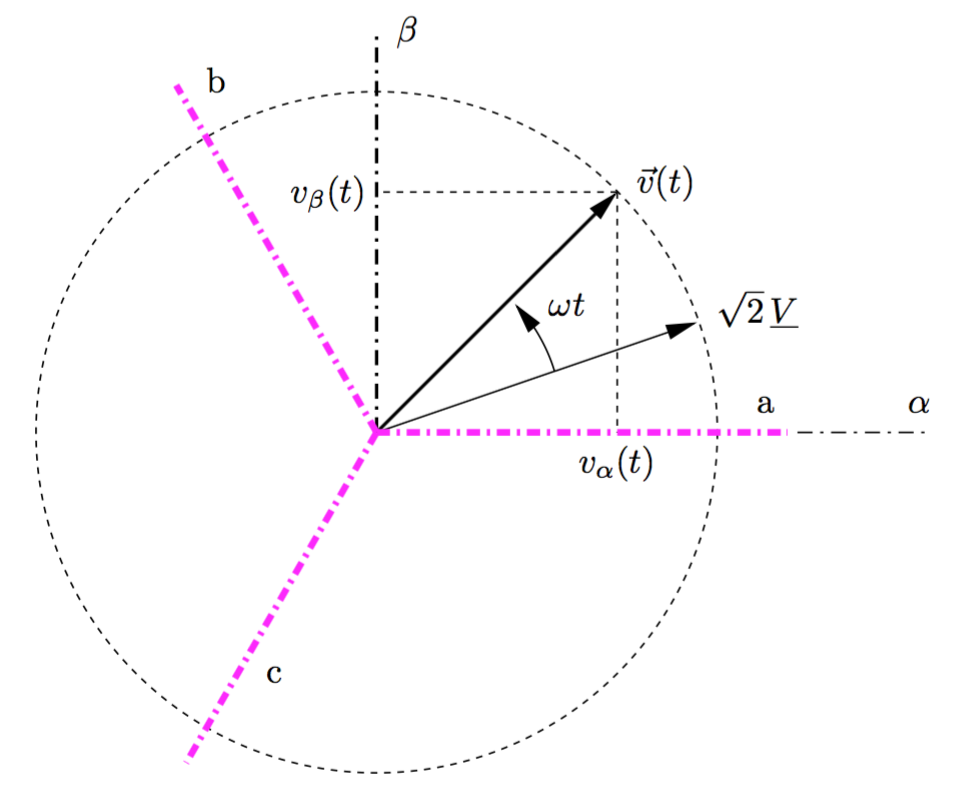
\includegraphics[scale=0.25]{ch4/26}
		\captionof{figure}{}
		\end{wrapfigure}
		$v(t)$ a donc une longueur constante $\sqrt{2}V$ qui est l'amplitude des tensions phase-neutre et tourne à une vitesse angulaire $\omega$. Le vecteur spatial est représenté ci-contre et l'extrémité parcourt un cercle de rayon $\hat{V} =\sqrt{2}V$ centré sur l'origine du plan complexe. \\\\\\\\\\
		
		\begin{wrapfigure}[6]{r}{4.5cm}
		\vspace{-5mm}
		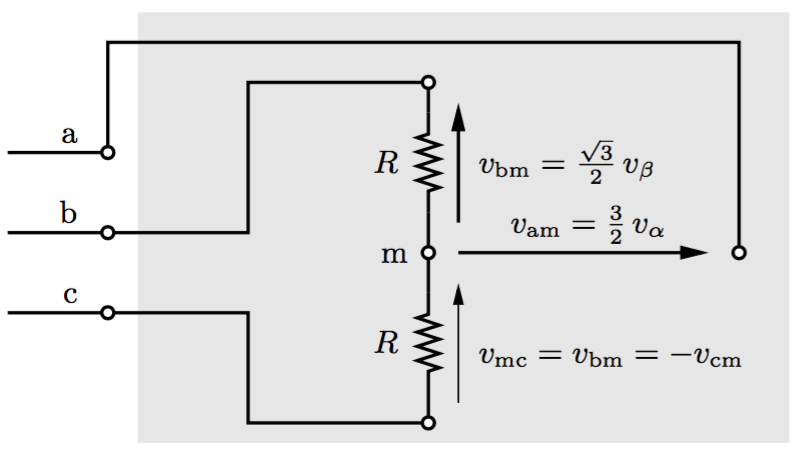
\includegraphics[scale=0.3]{ch4/27}
		\captionof{figure}{}
		\end{wrapfigure}
		\paragraph{Visualisation du vecteur spatial de tension à l'aide d'un oscilloscope} \quad En pratique, le circuit auxiliaire de la figure ci-contre permet d'obtenir les tensions $v_\alpha$ et $v_\beta$. $m$ est alors le point milieu d'un diviseur de tension (p.ex. résistif). On a alors que : 
		\begin{equation}
			v_{am} = \frac{3}{2}v_\alpha \qquad et \qquad v_{bm} = \frac{\sqrt{3}}{2}v_\beta . 
		\end{equation}
		Sur l'oscilloscope, en passant sous format XY, on peut obtenir un locus circulaire dans le cas particulier d'un régime sinusoïdal triphasé équilibré.
		
		\paragraph{Onduleur triphasé et l'hexagone de vecteurs spatiaux de tension} \quad L'onduleur de tension à 3 bras peut générer $2^3 = 8$ vecteurs spatiaux discrets et fixes selon la combinaison des interrupteurs. La figure ) gauche représente une des combinaisons possibles désignées par (010). On choisit pour $m$ le point milieu du bus DC. Le vecteur spatial est dans ce cas :
		\begin{equation}
			\vec{v} = \frac{2}{3} \frac{V_{dc}}{2}(-1 + 1e^{j2\pi /3}-1 e^{j2\pi /3}) = \frac{2}{3}V_{dc}e^{j2\pi /3}.
		\end{equation}
		On peut trouver ainsi les 6 vecteurs spatiaux non nuls suivants :
		\begin{equation}
			\vec{v}_k = \frac{2}{3}V_{dc}e^{j(k-1)\pi /3}\qquad avec \qquad 1\leq k \leq 6.
		\end{equation}
		Ils constituent les rayons d'un hexagone dans le plan complexe. Remarquons qu'on retrouve le schéma de commutation à onde carrée de la \autoref{fig:4.22} en parcourant les sommets de l'hexagone et en y restant pendant T/6. Les 2 vecteurs spatiaux restants sont nuls (interrupteurs supérieurs ou inférieurs tous fermés). 
		\begin{center}
		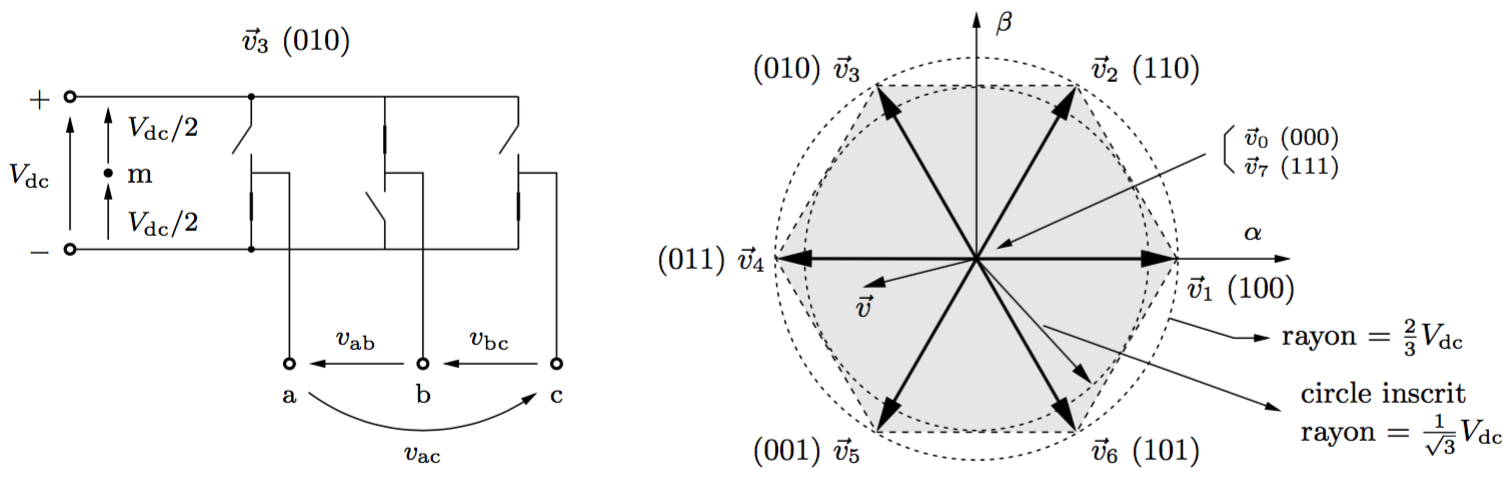
\includegraphics[scale=0.4]{ch4/29}
		\captionof{figure}{}
		\label{fig:4.27}
		\end{center}
		
		\paragraph{Modulation à vecteur spatial} \quad (SVM) permet de suivre en moyenne une consigne de vecteur spatial $\vec{v}(t)$, en considérant une certaine période de commutation $T_s$. Durant chaque $T_s$, selon le secteur d'hexagone dans lequel se trouve le $\vec{v}(t)$ souhaité, 4 des 8 vecteurs spatiaux sont combinés avec son poids adéquat. Par exemple, le vecteur $\vec{v}(t)$ de la \autoref{fig:4.27} s'obtient en combinant $\vec{v}, \vec{v}_5, \vec{v}_7 = 0$ et $\vec{v}_0 = 0$ : 
		\begin{equation}
			\vec{v} = \frac{T_4}{T_s}\vec{v}_4 + \frac{T_5}{T_s}\vec{v}_5 +\frac{T_7}{T_s}\vec{v}_7+ \frac{T_0}{T_s}\vec{v}_0
		\end{equation}
		avec $T_4+T_5+T_7+T_0=T_s$ et $T_7=T_0$. L'ordre dans lequel les 4 vecteurs sont commandés importe pour les pertes de commutation. On peut ainsi générer tout vecteur spatial $\vec{v}(t)$ toujours en moyenne à condition qu'il se trouve dans ou sur l'hexagone. Lorsque l'extrémité d'un $\vec{v}$ parcourt à vitesse constante une trajectoire circulaire à l'intérieur de l'hexagone, la tension de sortie de l'onduleur est dépourvue d'harmonique de faible rang. La valeur efficace maximum est obtenue en considérant le cercle inscrit dans l'hexagone, de rayon $\hat{V}_{1,max} = V_{dc}/\sqrt{3}$. 
		
		\paragraph{Plage de tension - comparaison avec MLI intersective} \quad Pour rappel, avec l'intersective, on évite les harmoniques de faible rang avec 3 $m(t)$ sinusoïdales d'amplitude max $\hat{m}=1$, avec tension max correspondante $\hat{V}_{1,max} = V_{dc}/2$. On peut toutefois aller au-delà de cette valeur en superposant un harmonique de rang 3 aux $m(t)$ sans faire apparaître des faibles rangs dans la tension de sortie ($\hat{V}_{1,max}=V_{dc}/\sqrt{3}$). Le tableau ci-dessous reprend les différentes modulations.
		\begin{center}
		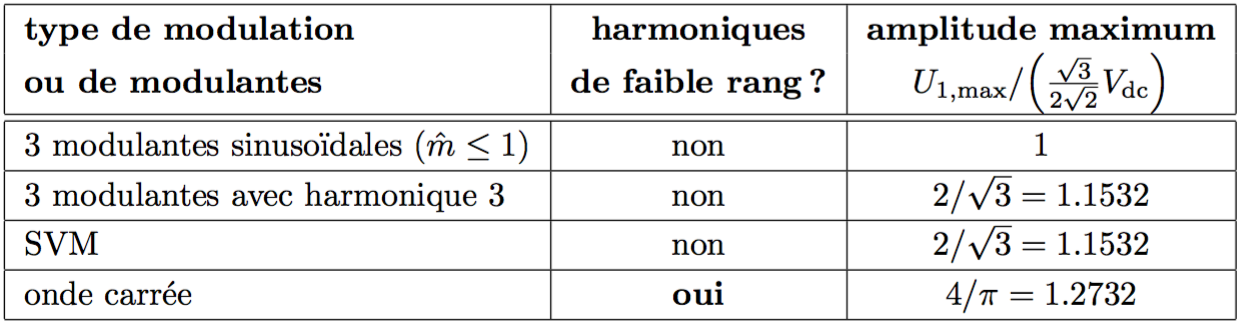
\includegraphics[scale=0.4]{ch4/30}
		\captionof{table}{}
		\end{center}
		
		Remarquons pour finir que la capacité en tension des interrupteurs dépend du bus $V_{dc}$ et non du schéma de commutation. 
		
\section{Commande en tension (par MLI) versus commande en courant (à hystérésis)}
	\paragraph{Convertisseurs de tension}\quad 
	Les ponts étudiés peuvent fonctionner en onduleur/redresseur et en hacheur. Comme l'alimentation se fait par tension DC, on peut directement commander les interrupteurs et la tension de sortie sera bien suivie en moyenne (mis à part les harmoniques de commutation) à condition de ne pas dépasser les limites imposées par le bus DC et la topologie du pont. Avec la MLI la commutation se fait à fréquence constante. 
	
	\paragraph{Entraînement électriques} \quad 
	La commande de tension peut convenir pour certains entraînements électriques en raison du lien, en régime établi, entre le niveau de tension et la fréquence dans le cas des machines à courant AC, et la vitesse de la machine. Les performances de ce type de commande sont médiocres. \\
	
	Pour de meilleures performances, il faut commander le \textbf{couple électromagnétique} instantané de la machine et donc les courants à y injecter. En prenant en compte les équations dynamiques de la machine, on peut traduire une consigne de couple en consigne de courant $i_{ref}$ (continu).
	
	\paragraph{Commande en tension}\quad 
	Pour la commande du courant, on passe soit par une commande (MLI ou autre, \autoref{fig:4.28}) de la tension, soit on agit directement sur les interrupteurs commandables du convertisseur en fonction de l'erreur du courant (hystérésis ou commande en courant, \autoref{fig:4.29}). 
	\begin{center}
	\begin{minipage}{0.49\textwidth}
	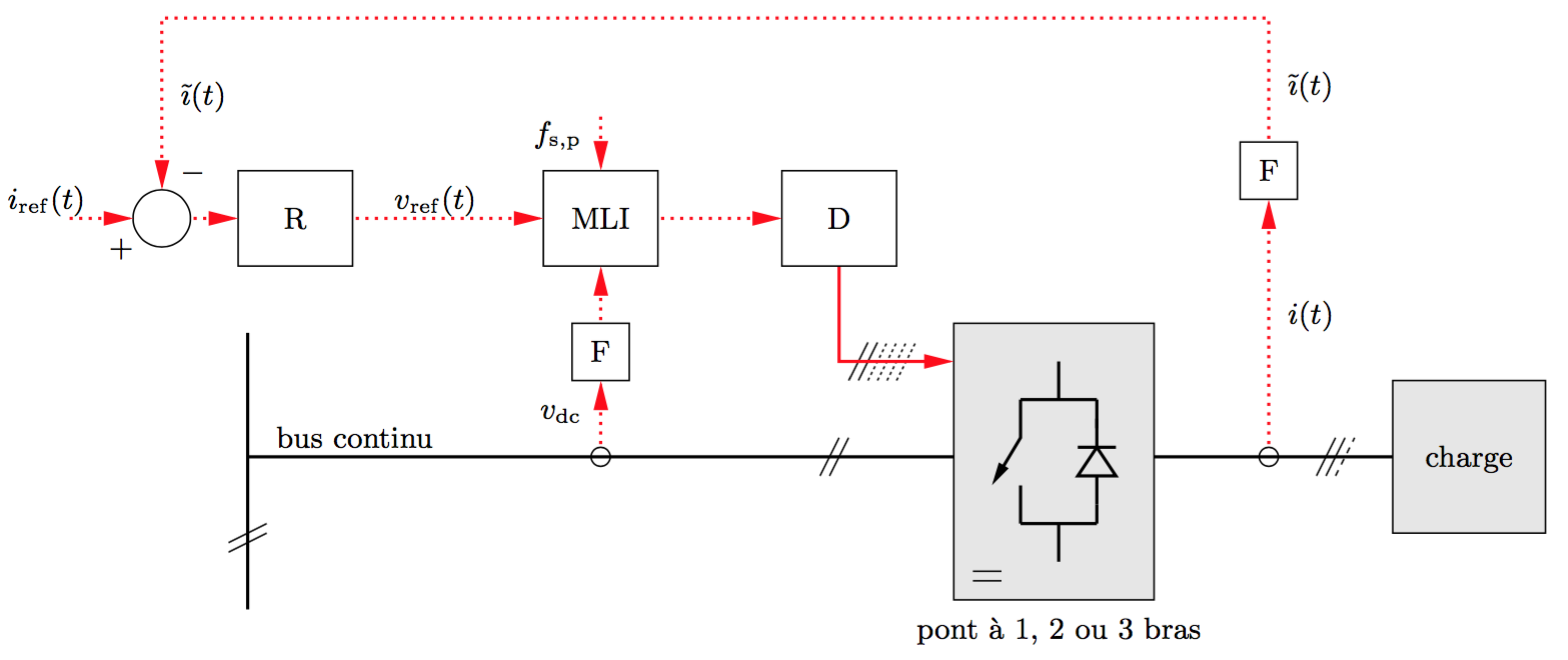
\includegraphics[scale=0.28]{ch4/31}
	\captionof{figure}{}
	\label{fig:4.28}
	\end{minipage}
	\begin{minipage}{0.49\textwidth}
	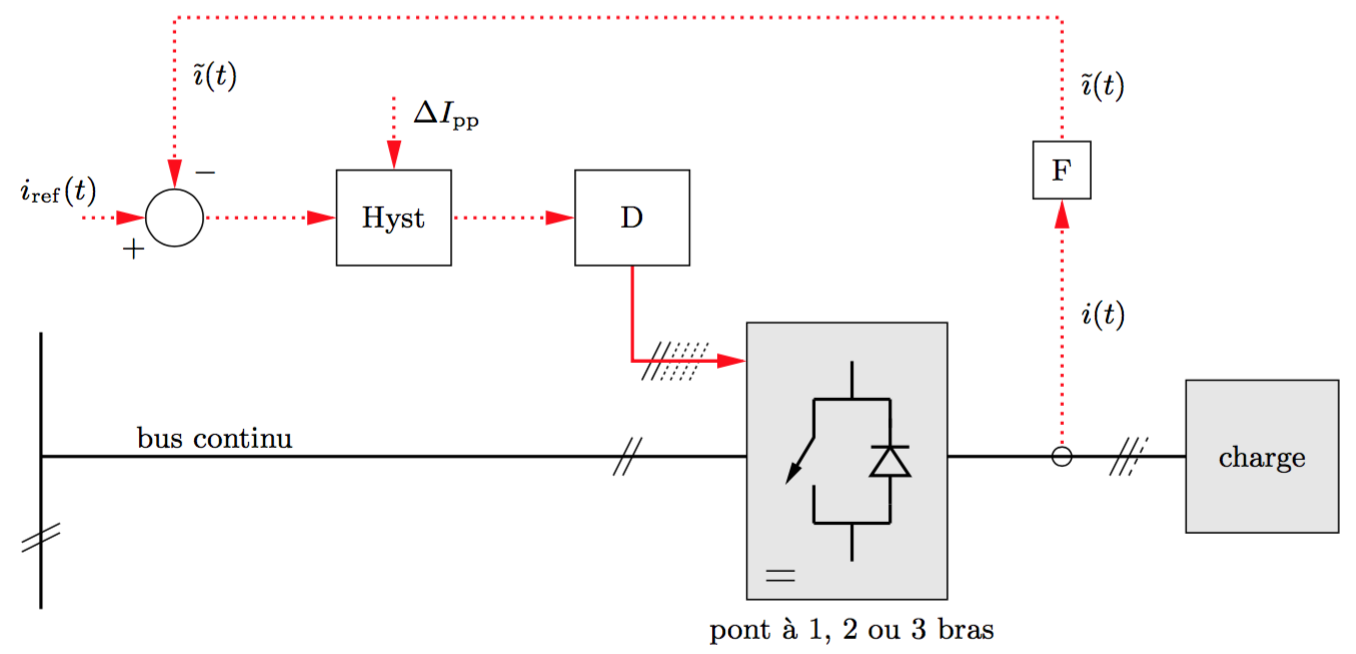
\includegraphics[scale=0.29]{ch4/32}
	\captionof{figure}{}
	\label{fig:4.29}
	\end{minipage}
	\end{center}
	
	Dans le premier cas, l'erreur de courant est traduite en une consigne de tension $v_{ref}$ via un bloc R régulateur, avant d'être réalisée par de la MLI intersective. La comparaison entre p(t) et le(s) m(t) se fait dans le bloc MLI et les \textbf{drivers de gâchettes} (D) se chargent de la commande des interrupteurs. Les \textbf{filtres passe-bas} (F) permettent de supprimer les harmoniques de commutation. 
	
	\paragraph{Commande en courant}\quad Dans ce cas, les interrupteurs sont directement commandés sur base de l'erreur de courant. Une \textbf{bande à hystérésis} $\Delta I_{pp}$ centrée autour de la consigne de courant est considérée. Si un bras fournit un courant qui dépasse la consigne de courant de plus de $\Delta I_{pp}/2$, l'interrupteur supérieur du bras est ouvert puis celui du bas fermé. Lorsqu'il descend ensuite en dessous de la limite inférieure de la bande, l'action inverse se produit. \\
	
	Cette commande est très simple, mais la fréquence de commutation n'est pas constante en raison de la dépendance aux paramètres du système (inductance) et $\Delta I_{pp}$. 
	
\section{Convertisseurs à source de courant}
	\begin{wrapfigure}[9]{l}{6.5cm}
		\vspace{-5mm}
		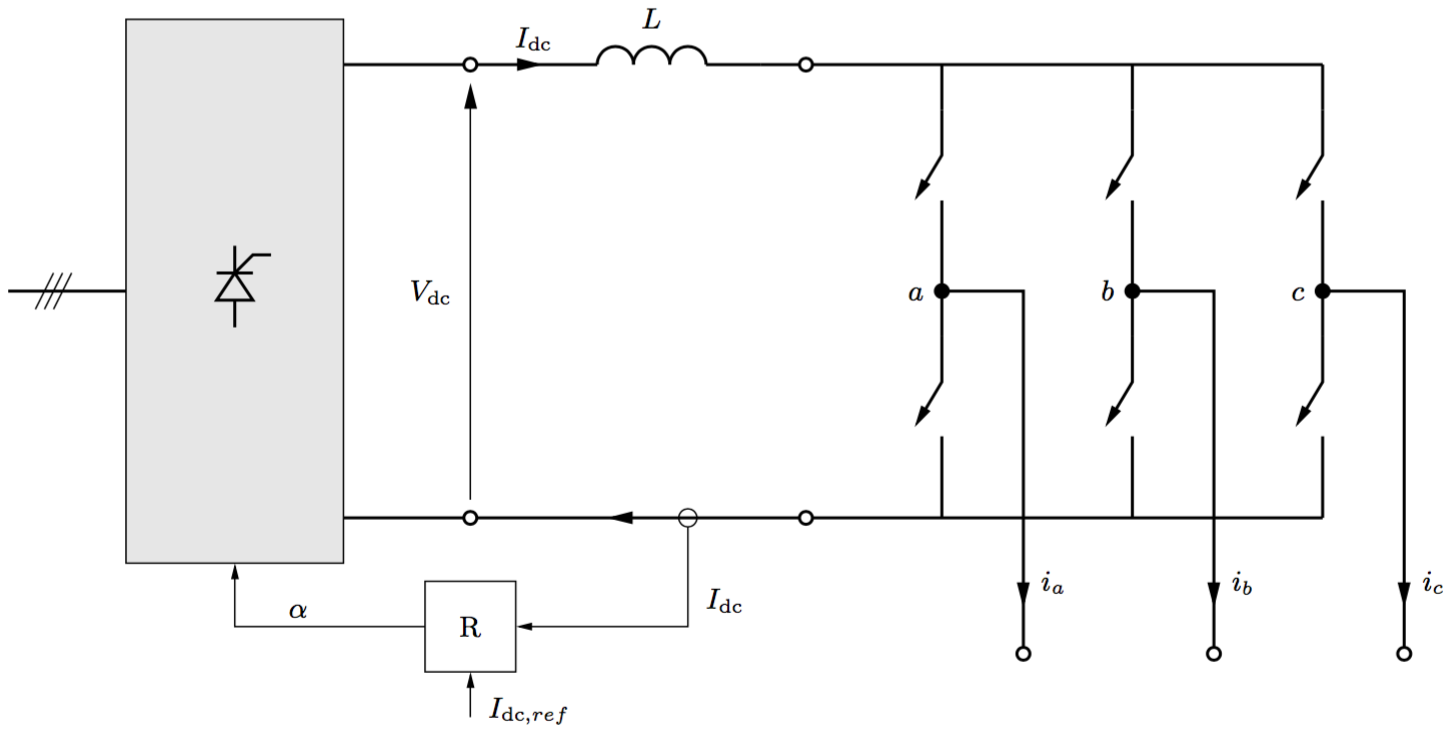
\includegraphics[scale=0.25]{ch4/33}
		\captionof{figure}{}
		\end{wrapfigure}
	On les utilise encore pour des applications de grade puissance et la commande à vitesse variable des grands moteurs asynchrones et synchrones. Un montage pratique est montré ci-contre. Le bus DC comprend une grande inductance L pour lisser $i_{dc}(t)$ unidirectionnel. Les GTO peuvent convenir comme interrupteurs dû à leur grande capacité en puissance. \\
	
	L'unidirectionallité de $i_{dc}(t)$ permet de se passer des diodes en antiparallèle. Un court-circuit du bras ne nécessite plus d'action ultrarapide de protection, ce grâce au grand L qui empêche une variation rapide du courant. Pour ces onduleurs, ce sont les circuits ouverts et la coupure du courant circulant dans L qui doivent être évités. Une commande en onde carrée permet d'utiliser des interrupteurs de faible capacité en fréquence, tels les GTO. \\
	
	Dans le système ci-contre, $I_{dc}$ est fourni par un redresseur à thyristor. En agissant sur $\alpha$, on règle $V_{dc}$ et donc $I_{dc}$. En inversant $V_{dc}$ on peut inverser le flux de puissance.
